% Chapter 5: Heavy tails and extreme value theory
% Statistics of Financial Markets -- Bachelor's programme, Bucharest University of Economic Studies
% GENERATED by latex/build_chapter5.py -- edit the generator, not this file.

\newcommand{\coursename}{Statistics of Financial Markets}
% Preambul comun SFM -- Statistica piețelor financiare / Statistics of Financial Markets (Beamer, 16:9)
% Același design ca MFM. Înainte de % Preambul comun SFM -- Statistica piețelor financiare / Statistics of Financial Markets (Beamer, 16:9)
% Același design ca MFM. Înainte de % Preambul comun SFM -- Statistica piețelor financiare / Statistics of Financial Markets (Beamer, 16:9)
% Același design ca MFM. Înainte de \input{../../latex/preamble} se definește
%   \newcommand{\coursename}{Statistics of Financial Markets}      (EN)
%   \newcommand{\coursename}{Statistica piețelor financiare}       (RO)  și  \def\sfmlang{ro}
% Fișierele .tex se află în EN/Courses, EN/Seminars, RO/Cursuri, RO/Seminarii (două niveluri sub rădăcină).
% Deck-urile sînt generate de latex/build_chapterN.py / build_seminarN.py (vezi latex/sfm_build.py).

\documentclass[9pt, aspectratio=169, t]{beamer}
\providecommand{\coursename}{Statistics of Financial Markets}

% Ensure content fits on slides
\setbeamersize{text margin left=8mm, text margin right=8mm}

%=============================================================================
% THEME AND STYLE CONFIGURATION
%=============================================================================
\usetheme{default}
% Using default theme for clean header/footer control

% Color Palette (matching Redispatch PDF)
\definecolor{MainBlue}{RGB}{26, 58, 110}
\definecolor{AccentBlue}{RGB}{26, 58, 110}
\definecolor{IDAred}{RGB}{205, 0, 0}
\definecolor{DarkGray}{RGB}{51, 51, 51}
\definecolor{MediumGray}{RGB}{128, 128, 128}
\definecolor{LightGray}{RGB}{248, 248, 248}
\definecolor{VeryLightGray}{RGB}{235, 235, 235}
\definecolor{KeynoteGray}{RGB}{218, 218, 218}
\definecolor{SectionGray}{RGB}{120, 120, 120}
\definecolor{FooterGray}{RGB}{100, 100, 100}
\definecolor{Crimson}{RGB}{220, 53, 69}
\definecolor{Forest}{RGB}{46, 125, 50}
\definecolor{Amber}{RGB}{181, 133, 63}
\definecolor{Orange}{RGB}{230, 126, 34}
\definecolor{Purple}{RGB}{142, 68, 173}

% Gradient background (exact Keynote 315° gradient: white to RGB 218,218,218)
\setbeamertemplate{background}{%
    \begin{tikzpicture}[remember picture, overlay]
        \shade[shading=axis, shading angle=315,
        top color=white, bottom color=KeynoteGray]
        (current page.south west) rectangle (current page.north east);
    \end{tikzpicture}%
}
% Fallback solid color for compatibility
\setbeamercolor{background canvas}{bg=}

\setbeamercolor{palette primary}{bg=MainBlue, fg=white}
\setbeamercolor{palette secondary}{bg=MainBlue!85, fg=white}
\setbeamercolor{palette tertiary}{bg=MainBlue!70, fg=white}
\setbeamercolor{structure}{fg=MainBlue}
\setbeamercolor{title}{fg=IDAred}
\setbeamercolor{frametitle}{fg=IDAred, bg=}
\setbeamercolor{block title}{bg=MainBlue, fg=white}
\setbeamercolor{block body}{bg=VeryLightGray, fg=DarkGray}
\setbeamercolor{block title alerted}{bg=Crimson, fg=white}
\setbeamercolor{block body alerted}{bg=Crimson!8, fg=DarkGray}
\setbeamercolor{block title example}{bg=Forest, fg=white}
\setbeamercolor{block body example}{bg=Forest!8, fg=DarkGray}
\setbeamercolor{item}{fg=MainBlue}

% Footer colors (override Madrid theme blue)
\setbeamercolor{author in head/foot}{fg=FooterGray, bg=}
\setbeamercolor{title in head/foot}{fg=FooterGray, bg=}
\setbeamercolor{date in head/foot}{fg=FooterGray, bg=}
\setbeamercolor{section in head/foot}{fg=FooterGray, bg=}
\setbeamercolor{subsection in head/foot}{fg=FooterGray, bg=}

% Bullet styles (apply everywhere including blocks)
\setbeamertemplate{itemize item}{\color{MainBlue}$\boxdot$}
\setbeamertemplate{itemize subitem}{\color{MainBlue}$\blacktriangleright$}
\setbeamertemplate{itemize subsubitem}{\color{MainBlue}\tiny$\bullet$}
\setbeamertemplate{itemize/enumerate body begin}{\normalsize}
\setbeamertemplate{itemize/enumerate subbody begin}{\normalsize}

% Item spacing - compact style
\setlength{\leftmargini}{10pt}       % Level 1: minimal indent
\setlength{\leftmarginii}{10pt}      % Level 2: minimal additional indent
% Compact list spacing (zero extra space before/after lists in blocks)
\makeatletter
\def\@listi{\leftmargin\leftmargini \topsep 0pt \parsep 0pt \itemsep 0pt}
\def\@listii{\leftmargin\leftmarginii \topsep 0pt \parsep 0pt \itemsep 0pt}
\makeatother

\setbeamertemplate{navigation symbols}{}

%=============================================================================
% CUSTOM HEADLINE
%=============================================================================
\setbeamertemplate{headline}{%
    \vskip10pt%
    \hbox to \paperwidth{%
        \hskip0.5cm%
        {\small\color{FooterGray}\renewcommand{\hyperlink}[2]{##2}\insertsectionhead}%
        \hfill%
        \textcolor{FooterGray}{\small\insertframenumber}%
        \hskip0.5cm%
    }%
    \vskip4pt%
    {\color{FooterGray}\hrule height 0.4pt}%
}

%=============================================================================
% CUSTOM FOOTER
%=============================================================================
\usepackage{fontawesome5}

\setbeamertemplate{footline}{%
    {\color{FooterGray}\hrule height 0.4pt}%
    \vskip4pt%
    \hbox to \paperwidth{%
        \hskip0.5cm%
        \textcolor{FooterGray}{\small\coursename}%
        \hfill%
        \raisebox{-0.1em}{%
            \begin{tikzpicture}[x=0.08em, y=0.08em, line width=0.4pt]
                \draw[FooterGray] (0,3) -- (1,4) -- (2,3.5) -- (3,5) -- (4,4) -- (5,6) -- (6,5.5) -- (7,4) -- (8,5) -- (9,7) -- (10,6) -- (11,5) -- (12,6.5) -- (13,8) -- (14,7) -- (15,6) -- (16,7.5) -- (17,9) -- (18,8) -- (19,7) -- (20,8.5) -- (21,10) -- (22,9) -- (23,8) -- (24,9.5);
            \end{tikzpicture}%
        }%
        \hskip0.5cm%
    }%
    \vskip6pt%
}

%=============================================================================
% PACKAGES
%=============================================================================
\usepackage[utf8]{inputenc}
\DeclareUnicodeCharacter{03B1}{\ensuremath{\alpha}}
\usepackage[T1]{fontenc}
\usepackage{amsmath, amssymb, amsthm}
\usepackage{mathtools}
\usepackage{bm}
\usepackage{tikz}
\usetikzlibrary{arrows.meta, positioning, shapes, calc, decorations.pathreplacing, shadings}
\usepackage{booktabs}
\usepackage{multirow}
\usepackage{array}
\usepackage{graphicx}
\usepackage{hyperref}
\usepackage{colortbl}
\usepackage{listings}
\lstset{language=Python, basicstyle=\ttfamily\scriptsize, keywordstyle=\color{MainBlue}\bfseries,
  commentstyle=\color{Forest}, stringstyle=\color{Crimson}, breaklines=true,
  frame=none, backgroundcolor=\color{VeryLightGray}, xleftmargin=2mm}
\hypersetup{colorlinks=true, linkcolor=MainBlue, urlcolor=MainBlue}
\graphicspath{{../../logos/}{../../charts/}{../../photos/}}
\usepackage{xcolor}
\hfuzz=2pt  % Suppress tiny overfull warnings (<2pt)
\vfuzz=2pt  % Suppress tiny vertical overfull warnings (<2pt)

%=============================================================================
% QUANTLET COMMANDS
%   \quantlet{<displayed name>}{<url>}       (generic, compatible with the older SFM decks)
%   \sfmquantlet{Ch_05}{SFM_ch5_garch}       -> https://github.com/danpele/SFM/tree/main/Quantlets/Ch_05/SFM_ch5_garch
%   \qlurl{<folder>} is defined per chapter by the generator (Quantlets/Ch_NN/<folder>)
%=============================================================================
\newcommand{\sfmrepo}{https://github.com/danpele/SFM}
\newcommand{\sfmqlbase}{https://github.com/danpele/SFM/tree/main/Quantlets}
\newcommand{\quantlet}[2]{%
    \hfill\href{#2}{%
        \raisebox{-0.15em}{
\includegraphics[height=0.7em]{ql_logo.png}}%
        \textcolor{MainBlue}{\tiny\ #1}%
    }%
}
\newcommand{\sfmquantlet}[2]{\quantlet{\detokenize{#2}}{\sfmqlbase/#1/#2}}

%=============================================================================
% NOTEBOOKS (Google Colab)
%   \colaburl{notebooks/EN/chapter5_seminar_notebook.ipynb} -> the Colab link of a file in the SFM repo
%   \nb: the chapter notebook (each seminar deck redefines it with \renewcommand)
%=============================================================================
\newcommand{\colaburl}[1]{https://colab.research.google.com/github/danpele/SFM/blob/main/#1}
\newcommand{\nb}{https://colab.research.google.com/github/danpele/SFM/tree/main/notebooks/EN}
\newcommand{\nbname}{notebooks/EN}

%=============================================================================
% SLIDE HELPERS (used by the generators; the same as in MFM)
%=============================================================================
% local font size for list bodies (the preamble forces \normalsize)
\newcommand{\itemsize}[1]{\setbeamertemplate{itemize/enumerate body begin}{#1}\setbeamertemplate{itemize/enumerate subbody begin}{#1}}
\newcommand{\intitle}[1]{{\hypersetup{urlcolor=white}#1}}   % white links inside coloured title bars
\newcommand{\imgcap}[1]{{\scriptsize #1}\\[0.5mm]}          % caption under a photo
\newcommand{\imgcredit}[2]{{\tiny\color{FooterGray}\href{#1}{#2}}}   % image credit: source URL, author/licence
\newcommand{\aiprompt}[1]{{\ttfamily\color{MainBlue}#1}}     % a prompt to an AI assistant

%=============================================================================
% SEMINARS: student version by default; the instructor wrapper *_solutions.tex sets \solutionstrue
%=============================================================================
\makeatletter\@ifundefined{ifsolutions}{\expandafter\newif\csname ifsolutions\endcsname}{}\makeatother
\newcommand{\solonly}[1]{\ifsolutions #1\fi}
\newcommand{\propsub}{\ifsolutions\else\framesubtitle{\ifdefined\sfmlang Rezolvarea se discută la seminar\else Solution discussed in class\fi}\fi}

%=============================================================================
% APPENDIX AND CHAPTER LINKS (latex/appendix_links.py writes the calls; it also re-declares these
% macros before \begin{document}, so the decks compile with or without this preamble block)
%=============================================================================
\providecommand{\sfmapplink}[3]{\hypertarget{#2}{}\hyperlink{#1}{\beamergotobutton{#3}}}
\providecommand{\sfmappback}[2]{\begin{tikzpicture}[remember picture,overlay]\node[anchor=south east] at ([xshift=-3mm,yshift=7mm]current page.south east){\hyperlink{#1}{\beamerreturnbutton{#2}}};\end{tikzpicture}}
\providecommand{\sfmchlink}[2]{\href{#1}{#2}}
\providecommand{\sfmchlinkt}[2]{\href{#1}{\usebeamercolor[fg]{frametitle}#2}}

%=============================================================================
% QUANTINAR COMMAND: link către un curs Quantinar (subiecte avansate)
%=============================================================================
\newcommand{\quantinar}[2]{%
    \href{#2}{%
        \raisebox{-0.15em}{
\includegraphics[height=0.8em]{qr_logo.png}}%
        \textcolor{MainBlue}{\scriptsize\ #1}%
    }%
}

%=============================================================================
% CUSTOM TITLE PAGE
%=============================================================================
\defbeamertemplate*{title page}{hybrid}[1][]
{
    \vspace{0.2cm}
    % Logos row - top header (with clickable links)
    \begin{center}
        \href{https://www.ase.ro}{
\includegraphics[height=1.0cm]{ase_logo.png}}\hspace{0.3cm}%
        \href{https://theida.net}{
\includegraphics[height=1.0cm]{ida_logo.png}}\hspace{0.3cm}%
        \href{https://blockchain-research-center.com}{
\includegraphics[height=1.0cm]{brc_logo.png}}\hspace{0.3cm}%
        \href{https://www.ai4efin.ase.ro}{
\includegraphics[height=1.0cm]{ai4efin_logo.png}}\hspace{0.3cm}%
        \href{https://ipe.ro/new}{
\includegraphics[height=1.0cm]{acad_logo.png}}\hspace{0.3cm}%
        \href{https://www.digital-finance-msca.com}{
\includegraphics[height=1.0cm]{msca_logo.png}}%
    \end{center}

    \vspace{0.6cm}

    % Main title with Q logos on sides (with clickable links)
    \begin{center}
        \begin{minipage}{0.1\textwidth}
            \centering
            \href{https://quantlet.com}{
\includegraphics[height=1.1cm]{ql_logo.png}}
        \end{minipage}%
        \begin{minipage}{0.78\textwidth}
            \centering
            {\LARGE\bfseries\usebeamercolor[fg]{title}\inserttitle}

            \vspace{0.3cm}

            {\usebeamerfont{subtitle}\usebeamercolor[fg]{title}\insertsubtitle}
        \end{minipage}%
        \begin{minipage}{0.1\textwidth}
            \centering
            \href{https://quantinar.com}{
\includegraphics[height=1.1cm]{qr_logo.png}}
        \end{minipage}
    \end{center}

    \vspace{0.6cm}

    % Authors (left aligned)
    \hspace{0.5cm}{\usebeamerfont{author}\insertauthor}

    \vspace{0.3cm}

    % Institute/Affiliations (left aligned)
    \hspace{0.5cm}\begin{minipage}[t]{0.9\textwidth}
        \raggedright\small\insertinstitute
    \end{minipage}
}

%=============================================================================
% THEOREM ENVIRONMENTS
%=============================================================================
\theoremstyle{definition}
\setbeamertemplate{theorems}[numbered]
\ifdefined\sfmlang
\newtheorem{defn}{Definiție}
\newtheorem{thm}{Teoremă}
\newtheorem{prop}{Propoziție}
\newtheorem{rmk}{Observație}
\else
\newtheorem{defn}{Definition}
\newtheorem{thm}{Theorem}
\newtheorem{prop}{Proposition}
\newtheorem{rmk}{Remark}
\fi

%=============================================================================
% CENTRED MINIPAGE (no extra vertical space)
%=============================================================================
\newenvironment{cminipage}[1]{%
    \par\noindent\hfill\begin{minipage}{#1}\ignorespaces
}{%
    \end{minipage}\hfill\null\par
}

%=============================================================================
% CUSTOM COMMANDS
%=============================================================================
\newcommand{\E}{\mathbb{E}}
\newcommand{\Var}{\text{Var}}
\newcommand{\Cov}{\text{Cov}}
\newcommand{\Corr}{\text{Corr}}
\newcommand{\R}{\mathbb{R}}
\newcommand{\N}{\mathbb{N}}
\newcommand{\Z}{\mathbb{Z}}
\newcommand{\B}{\mathbf{B}}
\newcommand{\imark}{\textcolor{MainBlue}{\textbullet}}
\newcommand{\RMSE}{\text{RMSE}}
\newcommand{\MAE}{\text{MAE}}
\newcommand{\MAPE}{\text{MAPE}}

 se definește
%   \newcommand{\coursename}{Statistics of Financial Markets}      (EN)
%   \newcommand{\coursename}{Statistica piețelor financiare}       (RO)  și  \def\sfmlang{ro}
% Fișierele .tex se află în EN/Courses, EN/Seminars, RO/Cursuri, RO/Seminarii (două niveluri sub rădăcină).
% Deck-urile sînt generate de latex/build_chapterN.py / build_seminarN.py (vezi latex/sfm_build.py).

\documentclass[9pt, aspectratio=169, t]{beamer}
\providecommand{\coursename}{Statistics of Financial Markets}

% Ensure content fits on slides
\setbeamersize{text margin left=8mm, text margin right=8mm}

%=============================================================================
% THEME AND STYLE CONFIGURATION
%=============================================================================
\usetheme{default}
% Using default theme for clean header/footer control

% Color Palette (matching Redispatch PDF)
\definecolor{MainBlue}{RGB}{26, 58, 110}
\definecolor{AccentBlue}{RGB}{26, 58, 110}
\definecolor{IDAred}{RGB}{205, 0, 0}
\definecolor{DarkGray}{RGB}{51, 51, 51}
\definecolor{MediumGray}{RGB}{128, 128, 128}
\definecolor{LightGray}{RGB}{248, 248, 248}
\definecolor{VeryLightGray}{RGB}{235, 235, 235}
\definecolor{KeynoteGray}{RGB}{218, 218, 218}
\definecolor{SectionGray}{RGB}{120, 120, 120}
\definecolor{FooterGray}{RGB}{100, 100, 100}
\definecolor{Crimson}{RGB}{220, 53, 69}
\definecolor{Forest}{RGB}{46, 125, 50}
\definecolor{Amber}{RGB}{181, 133, 63}
\definecolor{Orange}{RGB}{230, 126, 34}
\definecolor{Purple}{RGB}{142, 68, 173}

% Gradient background (exact Keynote 315° gradient: white to RGB 218,218,218)
\setbeamertemplate{background}{%
    \begin{tikzpicture}[remember picture, overlay]
        \shade[shading=axis, shading angle=315,
        top color=white, bottom color=KeynoteGray]
        (current page.south west) rectangle (current page.north east);
    \end{tikzpicture}%
}
% Fallback solid color for compatibility
\setbeamercolor{background canvas}{bg=}

\setbeamercolor{palette primary}{bg=MainBlue, fg=white}
\setbeamercolor{palette secondary}{bg=MainBlue!85, fg=white}
\setbeamercolor{palette tertiary}{bg=MainBlue!70, fg=white}
\setbeamercolor{structure}{fg=MainBlue}
\setbeamercolor{title}{fg=IDAred}
\setbeamercolor{frametitle}{fg=IDAred, bg=}
\setbeamercolor{block title}{bg=MainBlue, fg=white}
\setbeamercolor{block body}{bg=VeryLightGray, fg=DarkGray}
\setbeamercolor{block title alerted}{bg=Crimson, fg=white}
\setbeamercolor{block body alerted}{bg=Crimson!8, fg=DarkGray}
\setbeamercolor{block title example}{bg=Forest, fg=white}
\setbeamercolor{block body example}{bg=Forest!8, fg=DarkGray}
\setbeamercolor{item}{fg=MainBlue}

% Footer colors (override Madrid theme blue)
\setbeamercolor{author in head/foot}{fg=FooterGray, bg=}
\setbeamercolor{title in head/foot}{fg=FooterGray, bg=}
\setbeamercolor{date in head/foot}{fg=FooterGray, bg=}
\setbeamercolor{section in head/foot}{fg=FooterGray, bg=}
\setbeamercolor{subsection in head/foot}{fg=FooterGray, bg=}

% Bullet styles (apply everywhere including blocks)
\setbeamertemplate{itemize item}{\color{MainBlue}$\boxdot$}
\setbeamertemplate{itemize subitem}{\color{MainBlue}$\blacktriangleright$}
\setbeamertemplate{itemize subsubitem}{\color{MainBlue}\tiny$\bullet$}
\setbeamertemplate{itemize/enumerate body begin}{\normalsize}
\setbeamertemplate{itemize/enumerate subbody begin}{\normalsize}

% Item spacing - compact style
\setlength{\leftmargini}{10pt}       % Level 1: minimal indent
\setlength{\leftmarginii}{10pt}      % Level 2: minimal additional indent
% Compact list spacing (zero extra space before/after lists in blocks)
\makeatletter
\def\@listi{\leftmargin\leftmargini \topsep 0pt \parsep 0pt \itemsep 0pt}
\def\@listii{\leftmargin\leftmarginii \topsep 0pt \parsep 0pt \itemsep 0pt}
\makeatother

\setbeamertemplate{navigation symbols}{}

%=============================================================================
% CUSTOM HEADLINE
%=============================================================================
\setbeamertemplate{headline}{%
    \vskip10pt%
    \hbox to \paperwidth{%
        \hskip0.5cm%
        {\small\color{FooterGray}\renewcommand{\hyperlink}[2]{##2}\insertsectionhead}%
        \hfill%
        \textcolor{FooterGray}{\small\insertframenumber}%
        \hskip0.5cm%
    }%
    \vskip4pt%
    {\color{FooterGray}\hrule height 0.4pt}%
}

%=============================================================================
% CUSTOM FOOTER
%=============================================================================
\usepackage{fontawesome5}

\setbeamertemplate{footline}{%
    {\color{FooterGray}\hrule height 0.4pt}%
    \vskip4pt%
    \hbox to \paperwidth{%
        \hskip0.5cm%
        \textcolor{FooterGray}{\small\coursename}%
        \hfill%
        \raisebox{-0.1em}{%
            \begin{tikzpicture}[x=0.08em, y=0.08em, line width=0.4pt]
                \draw[FooterGray] (0,3) -- (1,4) -- (2,3.5) -- (3,5) -- (4,4) -- (5,6) -- (6,5.5) -- (7,4) -- (8,5) -- (9,7) -- (10,6) -- (11,5) -- (12,6.5) -- (13,8) -- (14,7) -- (15,6) -- (16,7.5) -- (17,9) -- (18,8) -- (19,7) -- (20,8.5) -- (21,10) -- (22,9) -- (23,8) -- (24,9.5);
            \end{tikzpicture}%
        }%
        \hskip0.5cm%
    }%
    \vskip6pt%
}

%=============================================================================
% PACKAGES
%=============================================================================
\usepackage[utf8]{inputenc}
\DeclareUnicodeCharacter{03B1}{\ensuremath{\alpha}}
\usepackage[T1]{fontenc}
\usepackage{amsmath, amssymb, amsthm}
\usepackage{mathtools}
\usepackage{bm}
\usepackage{tikz}
\usetikzlibrary{arrows.meta, positioning, shapes, calc, decorations.pathreplacing, shadings}
\usepackage{booktabs}
\usepackage{multirow}
\usepackage{array}
\usepackage{graphicx}
\usepackage{hyperref}
\usepackage{colortbl}
\usepackage{listings}
\lstset{language=Python, basicstyle=\ttfamily\scriptsize, keywordstyle=\color{MainBlue}\bfseries,
  commentstyle=\color{Forest}, stringstyle=\color{Crimson}, breaklines=true,
  frame=none, backgroundcolor=\color{VeryLightGray}, xleftmargin=2mm}
\hypersetup{colorlinks=true, linkcolor=MainBlue, urlcolor=MainBlue}
\graphicspath{{../../logos/}{../../charts/}{../../photos/}}
\usepackage{xcolor}
\hfuzz=2pt  % Suppress tiny overfull warnings (<2pt)
\vfuzz=2pt  % Suppress tiny vertical overfull warnings (<2pt)

%=============================================================================
% QUANTLET COMMANDS
%   \quantlet{<displayed name>}{<url>}       (generic, compatible with the older SFM decks)
%   \sfmquantlet{Ch_05}{SFM_ch5_garch}       -> https://github.com/danpele/SFM/tree/main/Quantlets/Ch_05/SFM_ch5_garch
%   \qlurl{<folder>} is defined per chapter by the generator (Quantlets/Ch_NN/<folder>)
%=============================================================================
\newcommand{\sfmrepo}{https://github.com/danpele/SFM}
\newcommand{\sfmqlbase}{https://github.com/danpele/SFM/tree/main/Quantlets}
\newcommand{\quantlet}[2]{%
    \hfill\href{#2}{%
        \raisebox{-0.15em}{
\includegraphics[height=0.7em]{ql_logo.png}}%
        \textcolor{MainBlue}{\tiny\ #1}%
    }%
}
\newcommand{\sfmquantlet}[2]{\quantlet{\detokenize{#2}}{\sfmqlbase/#1/#2}}

%=============================================================================
% NOTEBOOKS (Google Colab)
%   \colaburl{notebooks/EN/chapter5_seminar_notebook.ipynb} -> the Colab link of a file in the SFM repo
%   \nb: the chapter notebook (each seminar deck redefines it with \renewcommand)
%=============================================================================
\newcommand{\colaburl}[1]{https://colab.research.google.com/github/danpele/SFM/blob/main/#1}
\newcommand{\nb}{https://colab.research.google.com/github/danpele/SFM/tree/main/notebooks/EN}
\newcommand{\nbname}{notebooks/EN}

%=============================================================================
% SLIDE HELPERS (used by the generators; the same as in MFM)
%=============================================================================
% local font size for list bodies (the preamble forces \normalsize)
\newcommand{\itemsize}[1]{\setbeamertemplate{itemize/enumerate body begin}{#1}\setbeamertemplate{itemize/enumerate subbody begin}{#1}}
\newcommand{\intitle}[1]{{\hypersetup{urlcolor=white}#1}}   % white links inside coloured title bars
\newcommand{\imgcap}[1]{{\scriptsize #1}\\[0.5mm]}          % caption under a photo
\newcommand{\imgcredit}[2]{{\tiny\color{FooterGray}\href{#1}{#2}}}   % image credit: source URL, author/licence
\newcommand{\aiprompt}[1]{{\ttfamily\color{MainBlue}#1}}     % a prompt to an AI assistant

%=============================================================================
% SEMINARS: student version by default; the instructor wrapper *_solutions.tex sets \solutionstrue
%=============================================================================
\makeatletter\@ifundefined{ifsolutions}{\expandafter\newif\csname ifsolutions\endcsname}{}\makeatother
\newcommand{\solonly}[1]{\ifsolutions #1\fi}
\newcommand{\propsub}{\ifsolutions\else\framesubtitle{\ifdefined\sfmlang Rezolvarea se discută la seminar\else Solution discussed in class\fi}\fi}

%=============================================================================
% APPENDIX AND CHAPTER LINKS (latex/appendix_links.py writes the calls; it also re-declares these
% macros before \begin{document}, so the decks compile with or without this preamble block)
%=============================================================================
\providecommand{\sfmapplink}[3]{\hypertarget{#2}{}\hyperlink{#1}{\beamergotobutton{#3}}}
\providecommand{\sfmappback}[2]{\begin{tikzpicture}[remember picture,overlay]\node[anchor=south east] at ([xshift=-3mm,yshift=7mm]current page.south east){\hyperlink{#1}{\beamerreturnbutton{#2}}};\end{tikzpicture}}
\providecommand{\sfmchlink}[2]{\href{#1}{#2}}
\providecommand{\sfmchlinkt}[2]{\href{#1}{\usebeamercolor[fg]{frametitle}#2}}

%=============================================================================
% QUANTINAR COMMAND: link către un curs Quantinar (subiecte avansate)
%=============================================================================
\newcommand{\quantinar}[2]{%
    \href{#2}{%
        \raisebox{-0.15em}{
\includegraphics[height=0.8em]{qr_logo.png}}%
        \textcolor{MainBlue}{\scriptsize\ #1}%
    }%
}

%=============================================================================
% CUSTOM TITLE PAGE
%=============================================================================
\defbeamertemplate*{title page}{hybrid}[1][]
{
    \vspace{0.2cm}
    % Logos row - top header (with clickable links)
    \begin{center}
        \href{https://www.ase.ro}{
\includegraphics[height=1.0cm]{ase_logo.png}}\hspace{0.3cm}%
        \href{https://theida.net}{
\includegraphics[height=1.0cm]{ida_logo.png}}\hspace{0.3cm}%
        \href{https://blockchain-research-center.com}{
\includegraphics[height=1.0cm]{brc_logo.png}}\hspace{0.3cm}%
        \href{https://www.ai4efin.ase.ro}{
\includegraphics[height=1.0cm]{ai4efin_logo.png}}\hspace{0.3cm}%
        \href{https://ipe.ro/new}{
\includegraphics[height=1.0cm]{acad_logo.png}}\hspace{0.3cm}%
        \href{https://www.digital-finance-msca.com}{
\includegraphics[height=1.0cm]{msca_logo.png}}%
    \end{center}

    \vspace{0.6cm}

    % Main title with Q logos on sides (with clickable links)
    \begin{center}
        \begin{minipage}{0.1\textwidth}
            \centering
            \href{https://quantlet.com}{
\includegraphics[height=1.1cm]{ql_logo.png}}
        \end{minipage}%
        \begin{minipage}{0.78\textwidth}
            \centering
            {\LARGE\bfseries\usebeamercolor[fg]{title}\inserttitle}

            \vspace{0.3cm}

            {\usebeamerfont{subtitle}\usebeamercolor[fg]{title}\insertsubtitle}
        \end{minipage}%
        \begin{minipage}{0.1\textwidth}
            \centering
            \href{https://quantinar.com}{
\includegraphics[height=1.1cm]{qr_logo.png}}
        \end{minipage}
    \end{center}

    \vspace{0.6cm}

    % Authors (left aligned)
    \hspace{0.5cm}{\usebeamerfont{author}\insertauthor}

    \vspace{0.3cm}

    % Institute/Affiliations (left aligned)
    \hspace{0.5cm}\begin{minipage}[t]{0.9\textwidth}
        \raggedright\small\insertinstitute
    \end{minipage}
}

%=============================================================================
% THEOREM ENVIRONMENTS
%=============================================================================
\theoremstyle{definition}
\setbeamertemplate{theorems}[numbered]
\ifdefined\sfmlang
\newtheorem{defn}{Definiție}
\newtheorem{thm}{Teoremă}
\newtheorem{prop}{Propoziție}
\newtheorem{rmk}{Observație}
\else
\newtheorem{defn}{Definition}
\newtheorem{thm}{Theorem}
\newtheorem{prop}{Proposition}
\newtheorem{rmk}{Remark}
\fi

%=============================================================================
% CENTRED MINIPAGE (no extra vertical space)
%=============================================================================
\newenvironment{cminipage}[1]{%
    \par\noindent\hfill\begin{minipage}{#1}\ignorespaces
}{%
    \end{minipage}\hfill\null\par
}

%=============================================================================
% CUSTOM COMMANDS
%=============================================================================
\newcommand{\E}{\mathbb{E}}
\newcommand{\Var}{\text{Var}}
\newcommand{\Cov}{\text{Cov}}
\newcommand{\Corr}{\text{Corr}}
\newcommand{\R}{\mathbb{R}}
\newcommand{\N}{\mathbb{N}}
\newcommand{\Z}{\mathbb{Z}}
\newcommand{\B}{\mathbf{B}}
\newcommand{\imark}{\textcolor{MainBlue}{\textbullet}}
\newcommand{\RMSE}{\text{RMSE}}
\newcommand{\MAE}{\text{MAE}}
\newcommand{\MAPE}{\text{MAPE}}

 se definește
%   \newcommand{\coursename}{Statistics of Financial Markets}      (EN)
%   \newcommand{\coursename}{Statistica piețelor financiare}       (RO)  și  \def\sfmlang{ro}
% Fișierele .tex se află în EN/Courses, EN/Seminars, RO/Cursuri, RO/Seminarii (două niveluri sub rădăcină).
% Deck-urile sînt generate de latex/build_chapterN.py / build_seminarN.py (vezi latex/sfm_build.py).

\documentclass[9pt, aspectratio=169, t]{beamer}
\providecommand{\coursename}{Statistics of Financial Markets}

% Ensure content fits on slides
\setbeamersize{text margin left=8mm, text margin right=8mm}

%=============================================================================
% THEME AND STYLE CONFIGURATION
%=============================================================================
\usetheme{default}
% Using default theme for clean header/footer control

% Color Palette (matching Redispatch PDF)
\definecolor{MainBlue}{RGB}{26, 58, 110}
\definecolor{AccentBlue}{RGB}{26, 58, 110}
\definecolor{IDAred}{RGB}{205, 0, 0}
\definecolor{DarkGray}{RGB}{51, 51, 51}
\definecolor{MediumGray}{RGB}{128, 128, 128}
\definecolor{LightGray}{RGB}{248, 248, 248}
\definecolor{VeryLightGray}{RGB}{235, 235, 235}
\definecolor{KeynoteGray}{RGB}{218, 218, 218}
\definecolor{SectionGray}{RGB}{120, 120, 120}
\definecolor{FooterGray}{RGB}{100, 100, 100}
\definecolor{Crimson}{RGB}{220, 53, 69}
\definecolor{Forest}{RGB}{46, 125, 50}
\definecolor{Amber}{RGB}{181, 133, 63}
\definecolor{Orange}{RGB}{230, 126, 34}
\definecolor{Purple}{RGB}{142, 68, 173}

% Gradient background (exact Keynote 315° gradient: white to RGB 218,218,218)
\setbeamertemplate{background}{%
    \begin{tikzpicture}[remember picture, overlay]
        \shade[shading=axis, shading angle=315,
        top color=white, bottom color=KeynoteGray]
        (current page.south west) rectangle (current page.north east);
    \end{tikzpicture}%
}
% Fallback solid color for compatibility
\setbeamercolor{background canvas}{bg=}

\setbeamercolor{palette primary}{bg=MainBlue, fg=white}
\setbeamercolor{palette secondary}{bg=MainBlue!85, fg=white}
\setbeamercolor{palette tertiary}{bg=MainBlue!70, fg=white}
\setbeamercolor{structure}{fg=MainBlue}
\setbeamercolor{title}{fg=IDAred}
\setbeamercolor{frametitle}{fg=IDAred, bg=}
\setbeamercolor{block title}{bg=MainBlue, fg=white}
\setbeamercolor{block body}{bg=VeryLightGray, fg=DarkGray}
\setbeamercolor{block title alerted}{bg=Crimson, fg=white}
\setbeamercolor{block body alerted}{bg=Crimson!8, fg=DarkGray}
\setbeamercolor{block title example}{bg=Forest, fg=white}
\setbeamercolor{block body example}{bg=Forest!8, fg=DarkGray}
\setbeamercolor{item}{fg=MainBlue}

% Footer colors (override Madrid theme blue)
\setbeamercolor{author in head/foot}{fg=FooterGray, bg=}
\setbeamercolor{title in head/foot}{fg=FooterGray, bg=}
\setbeamercolor{date in head/foot}{fg=FooterGray, bg=}
\setbeamercolor{section in head/foot}{fg=FooterGray, bg=}
\setbeamercolor{subsection in head/foot}{fg=FooterGray, bg=}

% Bullet styles (apply everywhere including blocks)
\setbeamertemplate{itemize item}{\color{MainBlue}$\boxdot$}
\setbeamertemplate{itemize subitem}{\color{MainBlue}$\blacktriangleright$}
\setbeamertemplate{itemize subsubitem}{\color{MainBlue}\tiny$\bullet$}
\setbeamertemplate{itemize/enumerate body begin}{\normalsize}
\setbeamertemplate{itemize/enumerate subbody begin}{\normalsize}

% Item spacing - compact style
\setlength{\leftmargini}{10pt}       % Level 1: minimal indent
\setlength{\leftmarginii}{10pt}      % Level 2: minimal additional indent
% Compact list spacing (zero extra space before/after lists in blocks)
\makeatletter
\def\@listi{\leftmargin\leftmargini \topsep 0pt \parsep 0pt \itemsep 0pt}
\def\@listii{\leftmargin\leftmarginii \topsep 0pt \parsep 0pt \itemsep 0pt}
\makeatother

\setbeamertemplate{navigation symbols}{}

%=============================================================================
% CUSTOM HEADLINE
%=============================================================================
\setbeamertemplate{headline}{%
    \vskip10pt%
    \hbox to \paperwidth{%
        \hskip0.5cm%
        {\small\color{FooterGray}\renewcommand{\hyperlink}[2]{##2}\insertsectionhead}%
        \hfill%
        \textcolor{FooterGray}{\small\insertframenumber}%
        \hskip0.5cm%
    }%
    \vskip4pt%
    {\color{FooterGray}\hrule height 0.4pt}%
}

%=============================================================================
% CUSTOM FOOTER
%=============================================================================
\usepackage{fontawesome5}

\setbeamertemplate{footline}{%
    {\color{FooterGray}\hrule height 0.4pt}%
    \vskip4pt%
    \hbox to \paperwidth{%
        \hskip0.5cm%
        \textcolor{FooterGray}{\small\coursename}%
        \hfill%
        \raisebox{-0.1em}{%
            \begin{tikzpicture}[x=0.08em, y=0.08em, line width=0.4pt]
                \draw[FooterGray] (0,3) -- (1,4) -- (2,3.5) -- (3,5) -- (4,4) -- (5,6) -- (6,5.5) -- (7,4) -- (8,5) -- (9,7) -- (10,6) -- (11,5) -- (12,6.5) -- (13,8) -- (14,7) -- (15,6) -- (16,7.5) -- (17,9) -- (18,8) -- (19,7) -- (20,8.5) -- (21,10) -- (22,9) -- (23,8) -- (24,9.5);
            \end{tikzpicture}%
        }%
        \hskip0.5cm%
    }%
    \vskip6pt%
}

%=============================================================================
% PACKAGES
%=============================================================================
\usepackage[utf8]{inputenc}
\DeclareUnicodeCharacter{03B1}{\ensuremath{\alpha}}
\usepackage[T1]{fontenc}
\usepackage{amsmath, amssymb, amsthm}
\usepackage{mathtools}
\usepackage{bm}
\usepackage{tikz}
\usetikzlibrary{arrows.meta, positioning, shapes, calc, decorations.pathreplacing, shadings}
\usepackage{booktabs}
\usepackage{multirow}
\usepackage{array}
\usepackage{graphicx}
\usepackage{hyperref}
\usepackage{colortbl}
\usepackage{listings}
\lstset{language=Python, basicstyle=\ttfamily\scriptsize, keywordstyle=\color{MainBlue}\bfseries,
  commentstyle=\color{Forest}, stringstyle=\color{Crimson}, breaklines=true,
  frame=none, backgroundcolor=\color{VeryLightGray}, xleftmargin=2mm}
\hypersetup{colorlinks=true, linkcolor=MainBlue, urlcolor=MainBlue}
\graphicspath{{../../logos/}{../../charts/}{../../photos/}}
\usepackage{xcolor}
\hfuzz=2pt  % Suppress tiny overfull warnings (<2pt)
\vfuzz=2pt  % Suppress tiny vertical overfull warnings (<2pt)

%=============================================================================
% QUANTLET COMMANDS
%   \quantlet{<displayed name>}{<url>}       (generic, compatible with the older SFM decks)
%   \sfmquantlet{Ch_05}{SFM_ch5_garch}       -> https://github.com/danpele/SFM/tree/main/Quantlets/Ch_05/SFM_ch5_garch
%   \qlurl{<folder>} is defined per chapter by the generator (Quantlets/Ch_NN/<folder>)
%=============================================================================
\newcommand{\sfmrepo}{https://github.com/danpele/SFM}
\newcommand{\sfmqlbase}{https://github.com/danpele/SFM/tree/main/Quantlets}
\newcommand{\quantlet}[2]{%
    \hfill\href{#2}{%
        \raisebox{-0.15em}{
\includegraphics[height=0.7em]{ql_logo.png}}%
        \textcolor{MainBlue}{\tiny\ #1}%
    }%
}
\newcommand{\sfmquantlet}[2]{\quantlet{\detokenize{#2}}{\sfmqlbase/#1/#2}}

%=============================================================================
% NOTEBOOKS (Google Colab)
%   \colaburl{notebooks/EN/chapter5_seminar_notebook.ipynb} -> the Colab link of a file in the SFM repo
%   \nb: the chapter notebook (each seminar deck redefines it with \renewcommand)
%=============================================================================
\newcommand{\colaburl}[1]{https://colab.research.google.com/github/danpele/SFM/blob/main/#1}
\newcommand{\nb}{https://colab.research.google.com/github/danpele/SFM/tree/main/notebooks/EN}
\newcommand{\nbname}{notebooks/EN}

%=============================================================================
% SLIDE HELPERS (used by the generators; the same as in MFM)
%=============================================================================
% local font size for list bodies (the preamble forces \normalsize)
\newcommand{\itemsize}[1]{\setbeamertemplate{itemize/enumerate body begin}{#1}\setbeamertemplate{itemize/enumerate subbody begin}{#1}}
\newcommand{\intitle}[1]{{\hypersetup{urlcolor=white}#1}}   % white links inside coloured title bars
\newcommand{\imgcap}[1]{{\scriptsize #1}\\[0.5mm]}          % caption under a photo
\newcommand{\imgcredit}[2]{{\tiny\color{FooterGray}\href{#1}{#2}}}   % image credit: source URL, author/licence
\newcommand{\aiprompt}[1]{{\ttfamily\color{MainBlue}#1}}     % a prompt to an AI assistant

%=============================================================================
% SEMINARS: student version by default; the instructor wrapper *_solutions.tex sets \solutionstrue
%=============================================================================
\makeatletter\@ifundefined{ifsolutions}{\expandafter\newif\csname ifsolutions\endcsname}{}\makeatother
\newcommand{\solonly}[1]{\ifsolutions #1\fi}
\newcommand{\propsub}{\ifsolutions\else\framesubtitle{\ifdefined\sfmlang Rezolvarea se discută la seminar\else Solution discussed in class\fi}\fi}

%=============================================================================
% APPENDIX AND CHAPTER LINKS (latex/appendix_links.py writes the calls; it also re-declares these
% macros before \begin{document}, so the decks compile with or without this preamble block)
%=============================================================================
\providecommand{\sfmapplink}[3]{\hypertarget{#2}{}\hyperlink{#1}{\beamergotobutton{#3}}}
\providecommand{\sfmappback}[2]{\begin{tikzpicture}[remember picture,overlay]\node[anchor=south east] at ([xshift=-3mm,yshift=7mm]current page.south east){\hyperlink{#1}{\beamerreturnbutton{#2}}};\end{tikzpicture}}
\providecommand{\sfmchlink}[2]{\href{#1}{#2}}
\providecommand{\sfmchlinkt}[2]{\href{#1}{\usebeamercolor[fg]{frametitle}#2}}

%=============================================================================
% QUANTINAR COMMAND: link către un curs Quantinar (subiecte avansate)
%=============================================================================
\newcommand{\quantinar}[2]{%
    \href{#2}{%
        \raisebox{-0.15em}{
\includegraphics[height=0.8em]{qr_logo.png}}%
        \textcolor{MainBlue}{\scriptsize\ #1}%
    }%
}

%=============================================================================
% CUSTOM TITLE PAGE
%=============================================================================
\defbeamertemplate*{title page}{hybrid}[1][]
{
    \vspace{0.2cm}
    % Logos row - top header (with clickable links)
    \begin{center}
        \href{https://www.ase.ro}{
\includegraphics[height=1.0cm]{ase_logo.png}}\hspace{0.3cm}%
        \href{https://theida.net}{
\includegraphics[height=1.0cm]{ida_logo.png}}\hspace{0.3cm}%
        \href{https://blockchain-research-center.com}{
\includegraphics[height=1.0cm]{brc_logo.png}}\hspace{0.3cm}%
        \href{https://www.ai4efin.ase.ro}{
\includegraphics[height=1.0cm]{ai4efin_logo.png}}\hspace{0.3cm}%
        \href{https://ipe.ro/new}{
\includegraphics[height=1.0cm]{acad_logo.png}}\hspace{0.3cm}%
        \href{https://www.digital-finance-msca.com}{
\includegraphics[height=1.0cm]{msca_logo.png}}%
    \end{center}

    \vspace{0.6cm}

    % Main title with Q logos on sides (with clickable links)
    \begin{center}
        \begin{minipage}{0.1\textwidth}
            \centering
            \href{https://quantlet.com}{
\includegraphics[height=1.1cm]{ql_logo.png}}
        \end{minipage}%
        \begin{minipage}{0.78\textwidth}
            \centering
            {\LARGE\bfseries\usebeamercolor[fg]{title}\inserttitle}

            \vspace{0.3cm}

            {\usebeamerfont{subtitle}\usebeamercolor[fg]{title}\insertsubtitle}
        \end{minipage}%
        \begin{minipage}{0.1\textwidth}
            \centering
            \href{https://quantinar.com}{
\includegraphics[height=1.1cm]{qr_logo.png}}
        \end{minipage}
    \end{center}

    \vspace{0.6cm}

    % Authors (left aligned)
    \hspace{0.5cm}{\usebeamerfont{author}\insertauthor}

    \vspace{0.3cm}

    % Institute/Affiliations (left aligned)
    \hspace{0.5cm}\begin{minipage}[t]{0.9\textwidth}
        \raggedright\small\insertinstitute
    \end{minipage}
}

%=============================================================================
% THEOREM ENVIRONMENTS
%=============================================================================
\theoremstyle{definition}
\setbeamertemplate{theorems}[numbered]
\ifdefined\sfmlang
\newtheorem{defn}{Definiție}
\newtheorem{thm}{Teoremă}
\newtheorem{prop}{Propoziție}
\newtheorem{rmk}{Observație}
\else
\newtheorem{defn}{Definition}
\newtheorem{thm}{Theorem}
\newtheorem{prop}{Proposition}
\newtheorem{rmk}{Remark}
\fi

%=============================================================================
% CENTRED MINIPAGE (no extra vertical space)
%=============================================================================
\newenvironment{cminipage}[1]{%
    \par\noindent\hfill\begin{minipage}{#1}\ignorespaces
}{%
    \end{minipage}\hfill\null\par
}

%=============================================================================
% CUSTOM COMMANDS
%=============================================================================
\newcommand{\E}{\mathbb{E}}
\newcommand{\Var}{\text{Var}}
\newcommand{\Cov}{\text{Cov}}
\newcommand{\Corr}{\text{Corr}}
\newcommand{\R}{\mathbb{R}}
\newcommand{\N}{\mathbb{N}}
\newcommand{\Z}{\mathbb{Z}}
\newcommand{\B}{\mathbf{B}}
\newcommand{\imark}{\textcolor{MainBlue}{\textbullet}}
\newcommand{\RMSE}{\text{RMSE}}
\newcommand{\MAE}{\text{MAE}}
\newcommand{\MAPE}{\text{MAPE}}



\newcommand{\qlurl}[1]{https://github.com/danpele/SFM/tree/main/Quantlets/Ch_05/#1}

% Clickable citations (DOIs verified via Crossref)

\newcommand{\refHill}{\href{https://doi.org/10.1214/aos/1176343247}{Hill (1975)}}
\newcommand{\refFT}{\href{https://doi.org/10.1017/S0305004100015681}{Fisher \& Tippett (1928)}}
\newcommand{\refGnedenko}{\href{https://doi.org/10.2307/1968974}{Gnedenko (1943)}}
\newcommand{\refPickands}{\href{https://doi.org/10.1214/aos/1176343003}{Pickands (1975)}}
\newcommand{\refBdH}{\href{https://doi.org/10.1214/aop/1176996548}{Balkema \& de Haan (1974)}}
\newcommand{\refMF}{\href{https://doi.org/10.1016/S0927-5398(00)00012-8}{McNeil \& Frey (2000)}}
\newcommand{\refQRM}{\href{https://press.princeton.edu/books/hardcover/9780691166278/quantitative-risk-management}{McNeil, Frey \& Embrechts (2015)}}
\newcommand{\refEKM}{\href{https://doi.org/10.1007/978-3-642-33483-2}{Embrechts, Klüppelberg \& Mikosch (1997)}}
\newcommand{\refGumbel}{\href{https://doi.org/10.7312/gumb92958}{Gumbel (1958)}}
\newcommand{\refWeissman}{\href{https://doi.org/10.1080/01621459.1978.10480104}{Weissman (1978)}}
\newcommand{\refDS}{\href{https://doi.org/10.1111/j.2517-6161.1990.tb01796.x}{Davison \& Smith (1990)}}
\newcommand{\refColes}{\href{https://doi.org/10.1007/978-1-4471-3675-0}{Coles (2001)}}
\newcommand{\refGopi}{\href{https://doi.org/10.1103/PhysRevE.60.5305}{Gopikrishnan et al.\ (1999)}}
\newcommand{\refDdV}{\href{https://doi.org/10.1016/S0927-5398(97)00008-X}{Daníelsson \& de Vries (1997)}}
\newcommand{\refLongin}{\href{https://doi.org/10.1086/209695}{Longin (1996)}}
\newcommand{\refJdV}{\href{https://doi.org/10.2307/2109682}{Jansen \& de Vries (1991)}}
\newcommand{\refDRH}{\href{https://doi.org/10.1214/aos/1016120372}{Drees, Resnick \& de Haan (2000)}}
\newcommand{\refRocco}{\href{https://doi.org/10.1111/j.1467-6419.2012.00744.x}{Rocco (2014)}}
\newcommand{\refAT}{\href{https://doi.org/10.1016/S0378-4266(02)00283-2}{Acerbi \& Tasche (2002)}}
\newcommand{\refResnick}{\href{https://doi.org/10.1007/978-0-387-45024-7}{Resnick (2007)}}
\newcommand{\refJenkinson}{\href{https://doi.org/10.1002/qj.49708134804}{Jenkinson (1955)}}
\newcommand{\refPeleA}{\href{https://doi.org/10.3390/e21121204}{Pele, Lazar \& Mazurencu-Marinescu-Pele (2019)}}
\newcommand{\refPeleB}{\href{https://doi.org/10.3390/e19050226}{Pele, Lazar \& Dufour (2017)}}
\newcommand{\refFHH}{\href{https://doi.org/10.1007/978-3-030-13751-9}{Franke, Härdle \& Hafner (2019)}}
\newcommand{\refBHL}{\href{https://doi.org/10.1007/978-3-642-33929-5}{Borak, Härdle \& López-Cabrera (2013)}}
\newcommand{\refMandelbrot}{\href{https://doi.org/10.1086/294632}{Mandelbrot (1963)}}
\newcommand{\refCont}{\href{https://doi.org/10.1080/713665670}{Cont (2001)}}
\newcommand{\refWang}{\href{https://doi.org/10.1038/s41586-023-06221-2}{Wang et al.\ (2023)}}
\newcommand{\refCarlson}{\href{https://www.federalreserve.gov/pubs/feds/2007/200713/200713pap.pdf}{Carlson (2007)}}
\newcommand{\refBasel}{\href{https://www.bis.org/basel_framework/chapter/MAR/33.htm}{Basel Committee (MAR33)}}

\title[Statistics of Financial Markets]{Statistics of Financial Markets}
\subtitle{Chapter 5: Heavy tails and extreme value theory}
\author[D.T. Pele]{Daniel Traian PELE}
\institute{Bucharest University of Economic Studies\\
IDA Institute Digital Assets\\
Blockchain Research Center\\
AI4EFin Artificial Intelligence for Energy Finance\\
Romanian Academy, Institute for Economic Forecasting\\
MSCA Digital Finance}
\date{}

%=============================================================================
\providecommand{\sfmapplink}[3]{\hypertarget{#2}{}\hyperlink{#1}{\beamergotobutton{#3}}}  % APPLINKS-MACROS
\providecommand{\sfmappback}[2]{\begin{tikzpicture}[remember picture,overlay]\node[anchor=south east] at ([xshift=-3mm,yshift=7mm]current page.south east){\hyperlink{#1}{\beamerreturnbutton{#2}}};\end{tikzpicture}}  % APPLINKS-MACROS
\providecommand{\sfmchlink}[2]{\href{#1}{#2}}  % APPLINKS-MACROS
\providecommand{\sfmchlinkt}[2]{\href{#1}{\usebeamercolor[fg]{frametitle}#2}}  % APPLINKS-MACROS
\begin{document}
%=============================================================================

{
\setbeamertemplate{headline}{}
\setbeamertemplate{footline}{}
\begin{frame}[noframenumbering]
    \titlepage
\end{frame}
}
% BEGIN-ACRONYMS (generat de latex/acronyms.py; nu editati manual)
\begin{frame}{Acronyms used in this material}
\setbeamertemplate{itemize/enumerate body begin}{\tiny}
\begin{columns}[T]
\begin{column}{0.49\textwidth}
\begin{itemize}\setlength{\itemsep}{0pt}
    \item \textbf{AI}: Artificial Intelligence
    \item \textbf{BET}: Bucharest Exchange Trading (index)
    \item \textbf{BET-TR}: BET Total Return (index)
    \item \textbf{BVB}: Bursa de Valori București (the Bucharest Stock Exchange)
    \item \textbf{CI}: Confidence Interval
    \item \textbf{COVID-19}: COronaVIrus Disease 2019
    \item \textbf{EODHD}: EOD Historical Data (market-data provider)
    \item \textbf{ES}: Expected Shortfall
    \item \textbf{EVT}: Extreme Value Theory
    \item \textbf{GARCH}: Generalised AutoRegressive Conditional Heteroskedasticity
    \item \textbf{GEV}: Generalised Extreme Value (distribution)
    \item \textbf{GPD}: Generalised Pareto Distribution
    \item \textbf{ML}: Maximum Likelihood
\end{itemize}
\end{column}
\begin{column}{0.49\textwidth}
\begin{itemize}\setlength{\itemsep}{0pt}
    \item \textbf{OMV}: Österreichische Mineralölverwaltung (Austrian Mineral Oil Administration (OMV group))
    \item \textbf{POT}: Peaks Over Threshold
    \item \textbf{PP}: Probability–Probability (plot)
    \item \textbf{QQ}: Quantile–Quantile (plot)
    \item \textbf{SE}: Standard Error
    \item \textbf{SFE}: Statistics of Financial Markets, Exercises (Quantlet collection of the textbook)
\end{itemize}
\end{column}
\end{columns}
\end{frame}
% END-ACRONYMS

\begin{frame}{Today's Question and Route}
\itemsize{\small}
\begin{itemize}
    \item \textbf{Question}: how large can a daily loss be, and how often should we expect it?
    \begin{itemize}
        \item \sfmchlink{https://danpele.github.io/SFM/EN/Courses/chapter2_classical_distributions_stylised_facts.pdf}{Chapters 2} and \sfmchlink{https://danpele.github.io/SFM/EN/Courses/chapter3_alpha_stable_distributions.pdf}{3}: returns have heavier tails than the Normal distribution
        \item risk managers and regulators care about the tail, not about the centre
    \end{itemize}
    \item \textbf{Route} of the chapter
    \begin{itemize}
        \item three crashes: 1987, 2008, 2020
        \item heavy and light tails; regular variation and the tail index $\alpha$
        \item the Hill estimator and the mean excess function
        \item block maxima and the GEV distribution; peaks over threshold and the GPD
        \item VaR 1\%, ES 2.5\% and VaR 0.1\% by EVT, compared with historical simulation and the Normal distribution
    \end{itemize}
\end{itemize}
\end{frame}

\begin{frame}{Learning Outcomes}
\itemsize{\small}
\begin{itemize}
    \item Tell a heavy tail from a light tail and read a tail on log-log axes
    \item Estimate the tail index with the Hill estimator, with a standard error and a Hill plot
    \item State the Fisher--Tippett--Gnedenko and the Pickands--Balkema--de Haan theorems in words and in formulas
    \item Fit a GEV to block maxima and a GPD to the losses above a threshold; check the fit with PP and QQ plots
    \item Compute return levels, VaR and ES from an EVT fit, step by step
    \item Judge, on real data, when EVT improves on historical simulation and on the Normal distribution
\end{itemize}
\end{frame}

\begin{frame}{Reading and Tools}
\itemsize{\small}
\begin{itemize}
    \item Textbook: \refFHH, Ch.~18 (statistics of extreme risks)
    \begin{itemize}
        \item exercises with solutions: \refBHL, Ch.~18
    \end{itemize}
    \item Risk management view: \refQRM, Ch.~5 (extreme value theory)
    \item Reference books: \refEKM; \refColes
    \item Python Quantlets of this chapter: \href{https://github.com/danpele/SFM/tree/main/Quantlets/Ch_05}{Quantlets/Ch\_05}
    \begin{itemize}
        \item ported from the SFE Quantlets SFElshill, SFEhillquantile, SFEMeanExcessFun, SFEevt1, SFEtailGEV, SFEtailGPareto, block\_max and var\_pot
    \end{itemize}
    \item Lecture notebook: \href{\colaburl{notebooks/EN/chapter5_lecture_notebook.ipynb}}{open in Google Colab}
    \item Video course: \quantinar{Measuring Statistical Risk}{https://quantinar.com/course/100080/measuring-statistical-risk}
\end{itemize}
\end{frame}


%=============================================================================
\section{Why Tails Matter}
%=============================================================================

\begin{frame}{19 October 1987: Black Monday}
\itemsize{\small}
\begin{columns}[T]
\begin{column}{0.50\textwidth}
\begin{itemize}
    \item On 19 October 1987 the S\&P 500 fell about 20\% in one day \refCarlson
    \begin{itemize}
        \item as a log return: $\ln(1 - 0.20) = -22.3\%$
        \item larger than any daily loss in our data since 1990 (the worst: $-12.8\%$ on 16 March 2020)
    \end{itemize}
    \item Measure it with the Normal distribution fitted to the S\&P 500, 1990--2026
    \begin{itemize}
        \item daily standard deviation $\hat\sigma = 1.13\%$, so $z = -19.7$
        \item $P(Z \le -19.7) \approx 10^{-86}$: impossible, yet it happened
    \end{itemize}
    \item The Normal distribution says nothing useful about such days: we need a model of the tail
\end{itemize}
\end{column}
\begin{column}{0.46\textwidth}
\centering
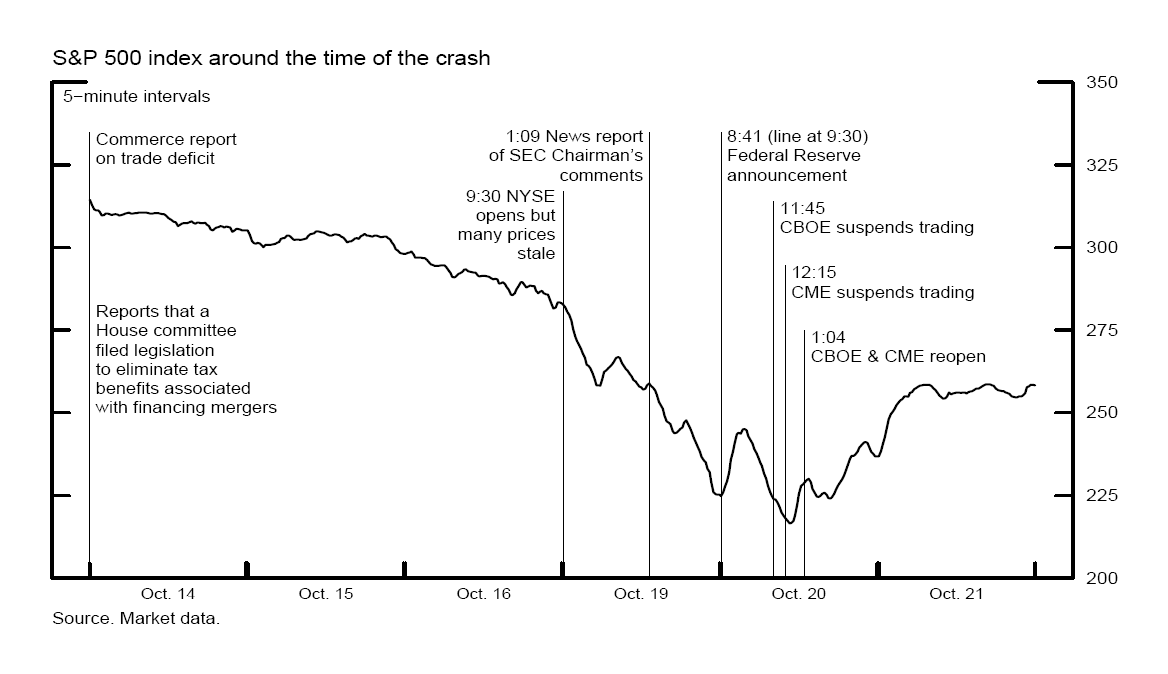
\includegraphics[height=0.38\textheight]{ch5_sp500_1987_fed.png}\\[1mm]
\imgcap{The S\&P 500, 14--21 October 1987, 5-minute data (Federal Reserve)}
\imgcredit{https://commons.wikimedia.org/wiki/File:S\%26P_500_index_around_the_time_of_the_crash.png}{Chart: M. Carlson, Federal Reserve Board (2006); public domain; Wikimedia Commons}
\end{column}
\end{columns}
\end{frame}

\begin{frame}{September 2008: Lehman Brothers}
\itemsize{\small}
\begin{columns}[T]
\begin{column}{0.60\textwidth}
\begin{itemize}
    \item Lehman Brothers filed for bankruptcy on 15 September 2008; the global financial crisis followed
    \begin{itemize}
        \item S\&P 500: $-9.5\%$ on 15 October 2008 and $-9.4\%$ on 1 December 2008
        \item BET: $-13.1\%$ on 7 January 2009
    \end{itemize}
    \item Large losses came in clusters, not one at a time
    \begin{itemize}
        \item volatility clustering (\sfmchlink{https://danpele.github.io/SFM/EN/Courses/chapter2_classical_distributions_stylised_facts.pdf}{Chapter 2}) concentrates the extremes in a few months
    \end{itemize}
    \item A VaR model based on the Normal distribution puts almost zero probability on such days
\end{itemize}
\end{column}
\begin{column}{0.36\textwidth}
\centering

\includegraphics[height=0.46\textheight]{ch5_lehman_2007.jpg}\\[1mm]
\imgcap{Lehman Brothers headquarters, New York, 2007}
\imgcredit{https://commons.wikimedia.org/wiki/File:Lehman_Brothers_Times_Square_by_David_Shankbone.jpg}{Photo: David Shankbone (2007); CC BY-SA 3.0; Wikimedia Commons}
\end{column}
\end{columns}
\end{frame}

\begin{frame}{March 2020: the COVID-19 Crash}
\itemsize{\small}
\begin{columns}[T]
\begin{column}{0.54\textwidth}
\begin{itemize}
    \item In one week of March 2020 three of our series had their largest daily loss
    \begin{itemize}
        \item S\&P 500: $-12.8\%$ on 16 March 2020
        \item DAX: $-13.1\%$ on 12 March 2020
        \item Bitcoin: $-46.5\%$ on 12 March 2020
    \end{itemize}
    \item The data of this chapter
    \begin{itemize}
        \item the data: daily closes from EODHD; S\&P 500 and DAX since 1990, BET since 1997, Bitcoin since 2014
    \end{itemize}
    \item Question of the chapter: how often should we expect such a day?
\end{itemize}
\end{column}
\begin{column}{0.42\textwidth}
\centering

\includegraphics[height=0.36\textheight]{ch5_fidi_2020.jpg}\\[1mm]
\imgcap{The empty Financial District of New York, 29 March 2020}
\imgcredit{https://commons.wikimedia.org/wiki/File:Solitude_(50073346382).jpg}{Photo: Billie Grace Ward (2020); CC BY 2.0; Wikimedia Commons}
\end{column}
\end{columns}
\end{frame}

\begin{frame}{Crash Days against the Normal Distribution}
\itemsize{\footnotesize}
\begin{center}
    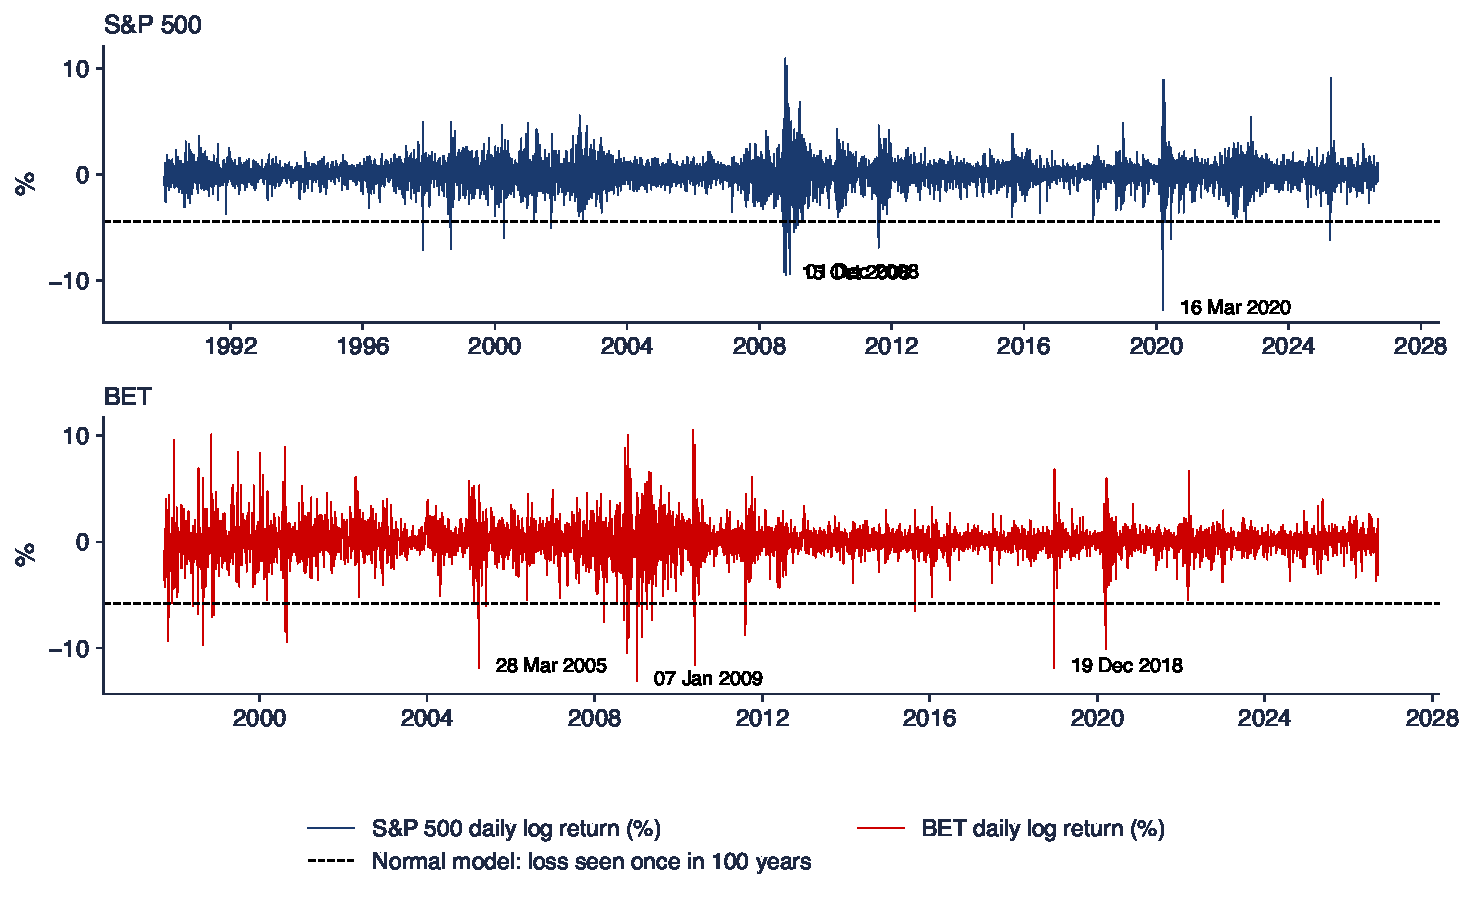
\includegraphics[width=0.97\textwidth,height=0.60\textheight,keepaspectratio]{sfm_ch5_crash_days.pdf}
\end{center}
\vspace{-0.25cm}
\begin{itemize}
    \item Dashed line: the daily loss that a Normal law fitted to each series exceeds once in 100 years (S\&P 500: $-4.4\%$; BET: $-5.8\%$)
    \item Observed: 35 such days for the S\&P 500 since 1990 and 34 for the BET since 1997
\end{itemize}
\quantlet{SFM\_ch5\_crashes}{\qlurl{SFM_ch5_crashes}}
\end{frame}

\begin{frame}{How Rare Are the Worst Days under the Normal Law?}
\itemsize{\footnotesize}
\begin{center}
\scriptsize
\begin{tabular}{llrrrrr}
\toprule
& worst day & loss (\%) & $z$ & Normal: once in (years) & days below $-4\sigma$ & expected \\
\midrule
S\&P 500 & 16 March 2020 & ${-12.8}$ & ${-11.3}$ & $10^{27}$ & 35 & $0.29$ \\
DAX & 12 March 2020 & ${-13.1}$ & ${-9.5}$ & $10^{19}$ & 27 & $0.29$ \\
BET & 7 January 2009 & ${-13.1}$ & ${-8.9}$ & $10^{16}$ & 33 & $0.23$ \\
Bitcoin & 12 March 2020 & ${-46.5}$ & ${-13.4}$ & $10^{38}$ & 18 & $0.14$ \\
\bottomrule
\end{tabular}
\end{center}
\begin{itemize}
    \item $z = (r - \hat\mu)/\hat\sigma$ with the mean and the standard deviation of the whole sample; once in $1/(p \times 252)$ years (365 days for Bitcoin)
    \item The Normal waiting times are absurd: far longer than the history of any market
    \item Losses beyond $4\sigma$: the Normal law expects fewer than one day per series; we see between 18 and 35
\end{itemize}\quantlet{SFM\_ch5\_crashes}{\qlurl{SFM_ch5_crashes}}
\end{frame}

\begin{frame}{Where Extreme Value Theory Comes From}
\itemsize{\small}
\begin{columns}[T]
\begin{column}{0.62\textwidth}
\begin{itemize}
    \item \textbf{EVT} (extreme value theory): the statistics of the largest values of a sample
    \begin{itemize}
        \item first used for floods, storms and the strength of materials
        \item \refGumbel: the yearly maximum of a river decides the height of a dam
    \end{itemize}
    \item In finance the same questions appear
    \begin{itemize}
        \item how large is the loss exceeded once in 10 years?
        \item how much capital covers the worst 1\% of days?
    \end{itemize}
    \item EVT models only the tail and lets the data speak there; early financial uses: \refJdV, \refLongin
\end{itemize}
\end{column}
\begin{column}{0.34\textwidth}
\centering
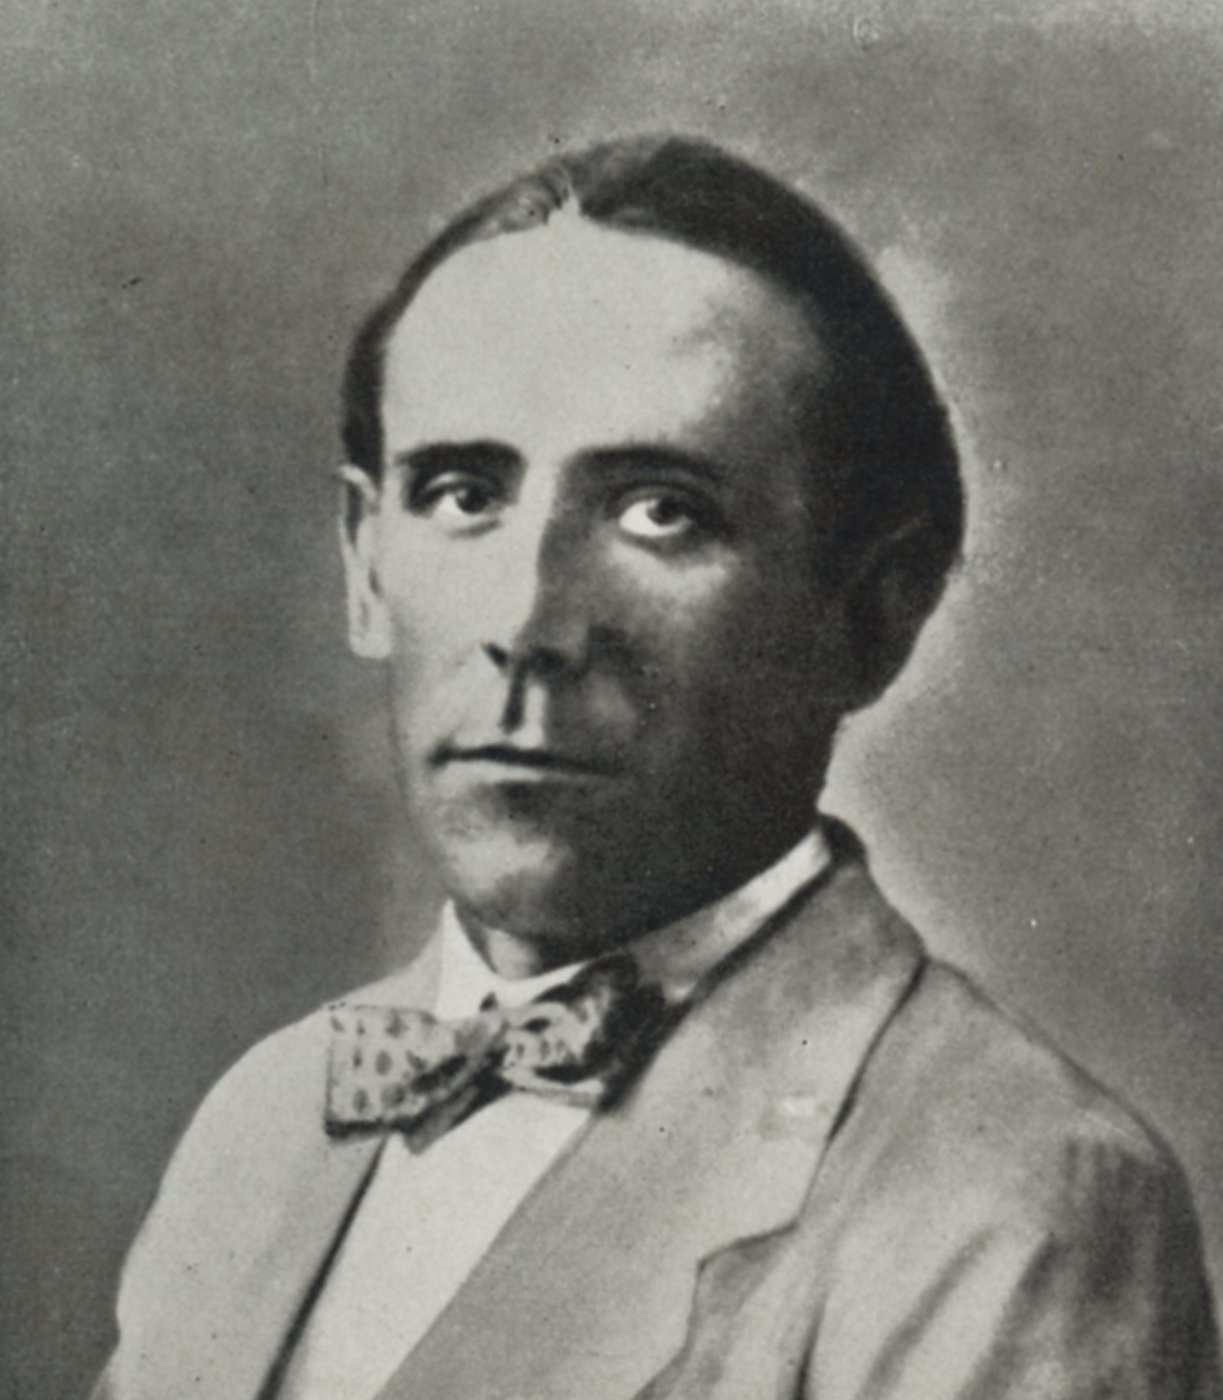
\includegraphics[height=0.44\textheight]{ch5_gumbel_1931.jpg}\\[1mm]
\imgcap{Emil Julius Gumbel (1891--1966)}
\imgcredit{https://commons.wikimedia.org/wiki/File:Emil_Julius_Gumbel.jpg}{Photo: unknown author (c. 1931); public domain; Wikimedia Commons}
\end{column}
\end{columns}
\end{frame}

\begin{frame}{Why the Tail Matters for Risk}
\itemsize{\small}
\begin{itemize}
    \item \textbf{VaR} (Value at Risk) at level $p$: the loss exceeded with probability $p$
    \begin{itemize}
        \item $\mathrm{VaR}_p = -q_p(r)$, with $q_p$ the $p$-quantile of the return; for example VaR 1\%
    \end{itemize}
    \item \textbf{ES} (expected shortfall) at level $p$: the average loss on the worst $p$ share of days
    \begin{itemize}
        \item $\mathrm{ES}_p = -E[r \mid r \le q_p(r)]$; banks report ES 2.5\% under the \refBasel
        \item ES looks inside the tail and is a coherent risk measure \refAT
    \end{itemize}
    \item Both live in the tail: a model that misses the tail misses the risk
    \item \textbf{Question for the room}: with 250 trading days a year, how many years of data contain about 10 days below VaR 0.1\%?
    \item \textbf{Answer}
    \begin{itemize}
        \item $10 / (0.001 \times 250) = 40$ years: historical data alone are too thin; EVT extrapolates the tail with a model
    \end{itemize}
\end{itemize}
\end{frame}

\begin{frame}{Recap: Why Tails Matter}
\itemsize{\small}
\begin{itemize}
    \item 1987, 2008, 2020: daily losses of 10--20\% for indices, almost 50\% for Bitcoin
    \item Under the Normal distribution these days should never happen
    \item VaR and ES are tail quantities; few observations lie that far out
    \item EVT: a theory for the shape of the tail, from hydrology to finance
\end{itemize}
\end{frame}


%=============================================================================
\section{Heavy Tails and Regular Variation}
%=============================================================================

\begin{frame}{Light and Heavy Tails}
\itemsize{\small}
\begin{itemize}
    \item Work with losses $L = -r$ (in \%): a large positive $L$ is a large loss
    \begin{itemize}
        \item the \textbf{tail} of $L$ is described by the survival function $\bar F(x) = P(L > x)$
    \end{itemize}
    \item \textbf{Light tail}: $\bar F(x)$ falls at least as fast as an exponential, $e^{-cx}$
    \begin{itemize}
        \item examples: Normal ($\bar F(x) \approx e^{-x^2/2}$), Exponential ($e^{-x}$); all moments are finite
    \end{itemize}
    \item \textbf{Heavy (power-law) tail}: $\bar F(x)$ falls like a power, $x^{-\alpha}$
    \begin{itemize}
        \item examples: Pareto, Student-t, the $\alpha$-stable laws of \sfmchlink{https://danpele.github.io/SFM/EN/Courses/chapter3_alpha_stable_distributions.pdf}{Chapter 3}
        \item $\alpha$ is the \textbf{tail index}: the smaller $\alpha$, the heavier the tail
    \end{itemize}
\end{itemize}
\end{frame}

\begin{frame}{Power Laws Fall Much More Slowly}
\itemsize{\footnotesize}
\begin{center}
    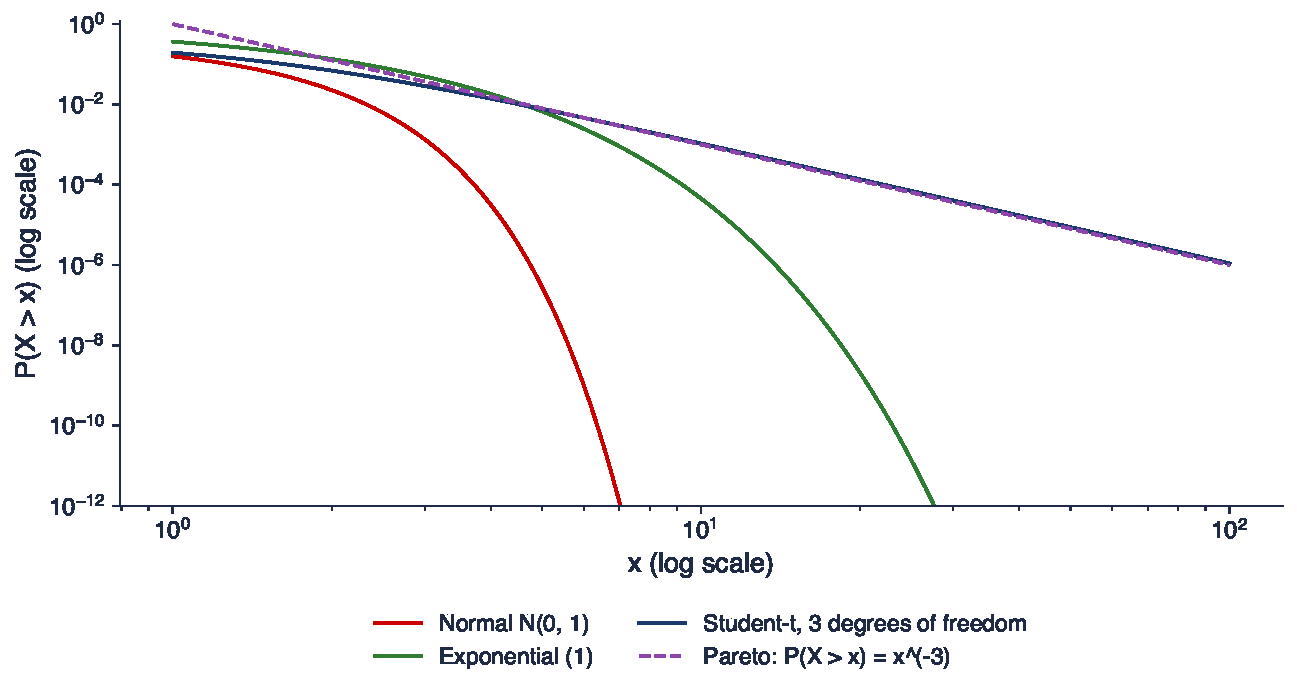
\includegraphics[width=0.97\textwidth,height=0.58\textheight,keepaspectratio]{sfm_ch5_light_heavy.pdf}
\end{center}
\vspace{-0.25cm}
\begin{itemize}
    \item On log-log axes a power law is a straight line with slope $-\alpha$; light tails bend down and vanish
    \item $P(X > 10)$: Normal $7.6\times 10^{-24}$, Exponential $4.5\times 10^{-5}$, Student-t with 3 degrees of freedom $1.1\times 10^{-3}$
\end{itemize}
\quantlet{SFM\_ch5\_tails\_loglog}{\qlurl{SFM_ch5_tails_loglog}}
\end{frame}

\begin{frame}{Regular Variation and the Tail Index}
\itemsize{\small}
\begin{itemize}
    \item $L$ has a \textbf{regularly varying} tail with index $\alpha > 0$ if $\bar F(x) = x^{-\alpha}\ell(x)$
    \begin{itemize}
        \item $\ell$ is \textbf{slowly varying}: $\ell(tx)/\ell(x) \to 1$ as $x \to \infty$, for every $t > 0$ (e.g.\ a constant, $\ln x$)
    \end{itemize}
    \item Equivalent: $\dfrac{P(L > tx)}{P(L > x)} \to t^{-\alpha}$ for large $x$
    \begin{itemize}
        \item doubling the loss divides its probability by $2^\alpha$, whatever the level
        \item Student-t with 3 degrees of freedom: $P(X > 20)/P(X > 10) = 0.128$, close to $2^{-3} = 0.125$
    \end{itemize}
    \item Tail indices of common laws
    \begin{itemize}
        \item Pareto with $\bar F(x) = (x/x_0)^{-\alpha}$: index $\alpha$; Student-t with $\nu$ degrees of freedom: $\alpha = \nu$
        \item $\alpha$-stable with $\alpha < 2$ (\sfmchlink{https://danpele.github.io/SFM/EN/Courses/chapter3_alpha_stable_distributions.pdf}{Chapter 3}): the same $\alpha$; Normal: no power tail ($\alpha = \infty$)
    \end{itemize}
\end{itemize}
\end{frame}

\begin{frame}{The Tail Index Decides Which Moments Exist}
\itemsize{\small}
\begin{itemize}
    \item For a regularly varying tail: $E|L|^m < \infty$ if $m < \alpha$ and $E|L|^m = \infty$ if $m > \alpha$
    \begin{itemize}
        \item $\alpha \le 1$: no mean; $\alpha \le 2$: no variance; $\alpha \le 4$: no kurtosis
    \end{itemize}
    \item The ``inverse cubic law'' of stock returns: $\alpha \approx 3$ \refGopi
    \begin{itemize}
        \item variance finite, kurtosis infinite: the sample kurtosis of \sfmchlink{https://danpele.github.io/SFM/EN/Courses/chapter2_classical_distributions_stylised_facts.pdf}{Chapter 2} does not settle
    \end{itemize}
    \item Link to \sfmchlink{https://danpele.github.io/SFM/EN/Courses/chapter3_alpha_stable_distributions.pdf}{Chapter 3}
    \begin{itemize}
        \item the stable $\alpha$ ($\approx 1.5$) is fitted to the whole distribution; the tail index here uses only the tail
        \item a tail index near 3 is the evidence against infinite variance announced in \sfmchlink{https://danpele.github.io/SFM/EN/Courses/chapter3_alpha_stable_distributions.pdf}{Chapter 3} \refMandelbrot
    \end{itemize}
\end{itemize}
\end{frame}

\begin{frame}{Real Losses on Log-Log Axes}
\itemsize{\footnotesize}
\begin{center}
    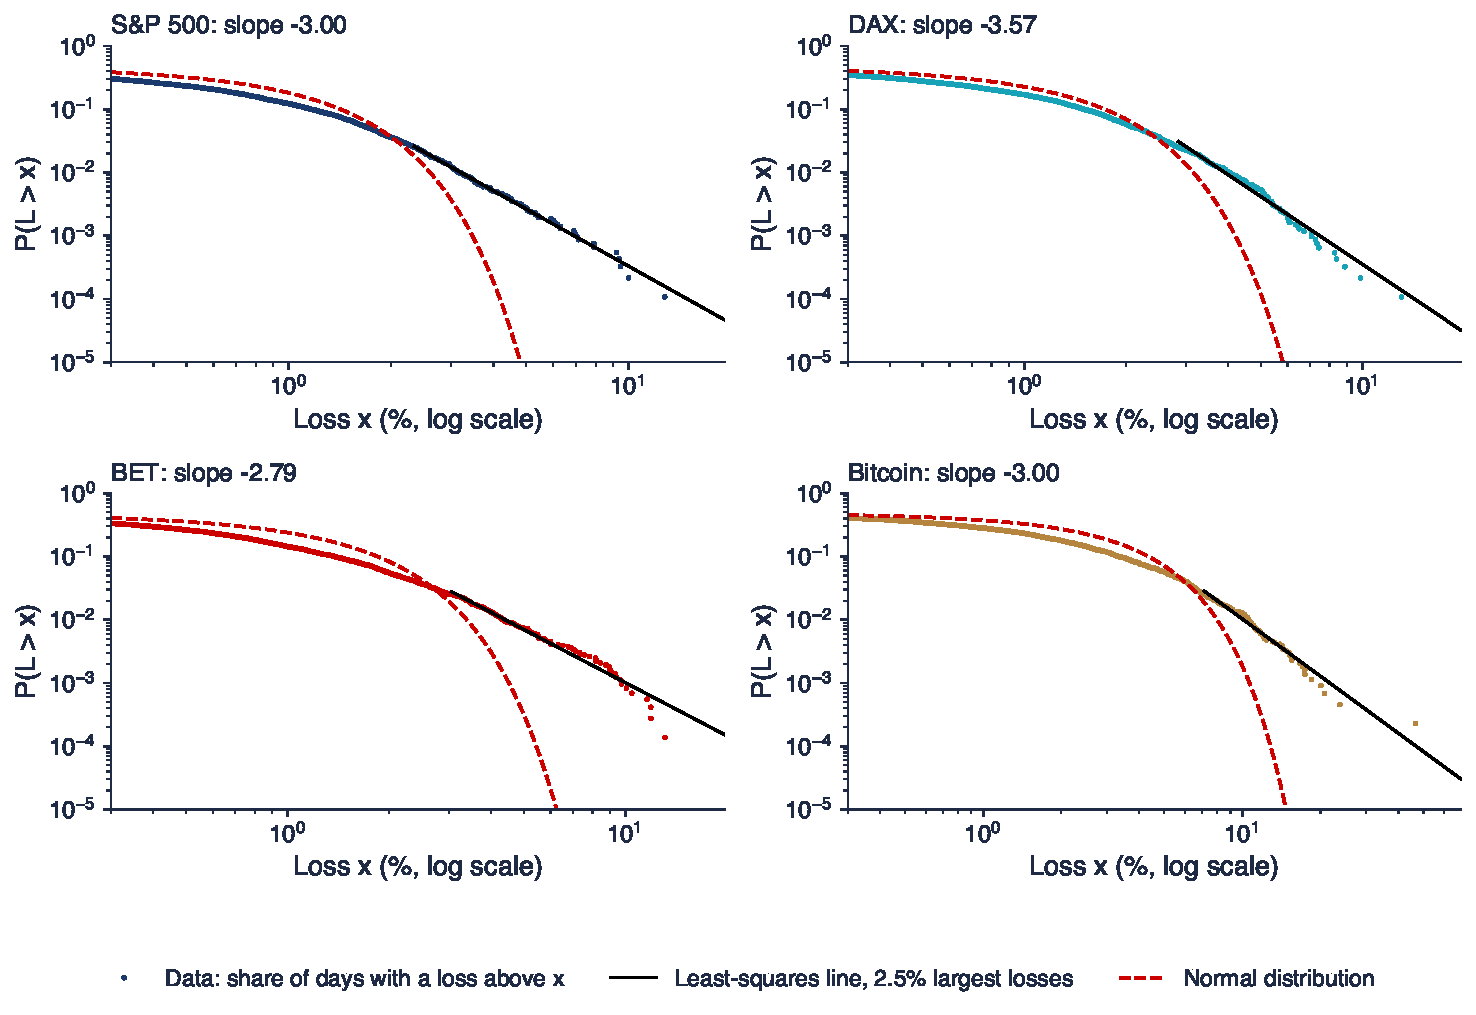
\includegraphics[width=0.97\textwidth,height=0.64\textheight,keepaspectratio]{sfm_ch5_loglog_real.pdf}
\end{center}
\vspace{-0.25cm}
\begin{itemize}
    \item Dots: the share of days with a loss above $x$; black: least-squares line through the 2.5\% largest losses; red: Normal
    \item Slopes: S\&P 500 $-3.00$, DAX $-3.57$, BET $-2.79$, Bitcoin $-3.00$: straight lines, power tails
\end{itemize}
\quantlet{SFM\_ch5\_tails\_loglog}{\qlurl{SFM_ch5_tails_loglog}}
\end{frame}

\begin{frame}{Reading a Log-Log Tail Plot}
\itemsize{\small}
\begin{itemize}
    \item If $\bar F(x) \approx C x^{-\alpha}$, then $\ln \bar F(x) \approx \ln C - \alpha \ln x$: a line with slope $-\alpha$
    \begin{itemize}
        \item \textbf{least-squares estimator}: regress $\ln(i/n)$ on $\ln L_{(i)}$ for the $k$ largest losses $L_{(1)} \ge \dots \ge L_{(k)}$
        \item $L_{(i)}$ is the $i$-th largest loss, an \textbf{order statistic}
    \end{itemize}
    \item The body of the distribution (small losses) bends away from the line: the power law holds only in the tail
    \item The Normal tail drops below the data already at 3--4\% for the indices
    \item The least-squares slope is simple but its points are not independent; the Hill estimator is the standard tool
\end{itemize}\quantlet{SFM\_ch5\_tails\_loglog}{\qlurl{SFM_ch5_tails_loglog}}
\end{frame}

\begin{frame}{Worked Example: a Pareto Tail}
\itemsize{\small}
\begin{itemize}
    \item Daily losses have a Pareto tail with $\alpha = 3$ and $P(L > 3\%) = 1\%$
    \begin{itemize}
        \item $P(L > x) = 1\% \times (x/3)^{-3}$ for $x \ge 3\%$
    \end{itemize}
    \item Loss above 6\%: $1\% \times 2^{-3} = 0.125\%$; above 9\%: $1\% \times 3^{-3} = 0.037\%$
    \begin{itemize}
        \item doubling the loss divides the probability by $2^3 = 8$
    \end{itemize}
    \item \textbf{What do you think?} Which loss is exceeded with probability 0.1\% (VaR 0.1\%)?
    \item \textbf{Answer}
    \begin{itemize}
        \item solve $1\% \times (x/3)^{-3} = 0.1\%$: $x = 3 \times 10^{1/3} = 3 \times 2.15 = 6.46\%$
        \item a probability ten times smaller only moves the loss by a factor $10^{1/\alpha}$
    \end{itemize}
\end{itemize}
\end{frame}

\begin{frame}{Recap: Heavy Tails}
\itemsize{\small}
\begin{itemize}
    \item Heavy tail: $P(L > x) = x^{-\alpha}\ell(x)$, a straight line on log-log axes
    \item The tail index $\alpha$ decides which moments exist: moments of order below $\alpha$
    \item Daily index losses: slopes near 3, the inverse cubic law
    \item Power law: the VaR moves only by $10^{1/\alpha}$ when the probability falls tenfold
\end{itemize}
\end{frame}


%=============================================================================
\section{The Hill Estimator}
%=============================================================================

\begin{frame}{The Hill Estimator}
\itemsize{\small}
\begin{itemize}
    \item Sort the losses: $L_{(1)} \ge L_{(2)} \ge \dots \ge L_{(n)}$; keep the $k$ largest
    \begin{itemize}
        \item \textbf{Hill estimator} \refHill: $\hat\alpha_k = \Big[\dfrac{1}{k}\sum_{i=1}^{k}\ln\dfrac{L_{(i)}}{L_{(k+1)}}\Big]^{-1}$
        \item the threshold is the $(k+1)$-th largest loss, $u = L_{(k+1)}$
    \end{itemize}
    \item Why it works: if $P(L > x \mid L > u) = (x/u)^{-\alpha}$ (Pareto above $u$), then $\ln(L/u)$ given $L > u$ is Exponential with mean $1/\alpha$
    \begin{itemize}
        \item the mean of the $k$ log excesses estimates $1/\alpha$; its inverse estimates $\alpha$
        \item Hill $=$ the maximum likelihood estimator of a Pareto tail above $u$
    \end{itemize}
    \item Ported from the SFE Quantlet SFElshill (least-squares and Hill estimators of the tail index) \refFHH
\end{itemize}
\end{frame}

\begin{frame}{Worked Example: Hill on Six Losses}
\itemsize{\small}
\begin{itemize}
    \item The six largest daily losses (\%): $9.5, 7.2, 6.1, 5.4, 4.8, 4.0$; take $k = 5$, so $L_{(6)} = 4.0$
    \item Log excesses $\ln(L_{(i)}/4.0)$
    \begin{itemize}
        \item $0.865$, $0.588$, $0.422$, $0.300$, $0.182$; mean $0.471$
    \end{itemize}
    \item $\hat\alpha_5 = 1/0.471 = 2.12$
    \item Standard error under independence: $\mathrm{SE}(\hat\alpha) \approx \hat\alpha/\sqrt{k} = 0.95$
    \begin{itemize}
        \item with $k = 5$ the estimate is very imprecise: real applications use hundreds of losses
    \end{itemize}
\end{itemize}
\end{frame}

\begin{frame}{Choosing $k$: the Hill Plot}
\itemsize{\small}
\begin{itemize}
    \item \textbf{Small $k$}: only the far tail, few points: high variance
    \item \textbf{Large $k$}: the body of the distribution enters, where the power law fails: bias
    \item The \textbf{Hill plot}: $\hat\alpha_k$ against $k$; look for a region where it is flat \refDRH
    \begin{itemize}
        \item here $k$ is shown as a share of the sample, $k/n$ between 0.5\% and 10\%
    \end{itemize}
    \item Fix the rule before looking at the result: here $k = 2.5\%$ of $n$
    \begin{itemize}
        \item and report the estimates at $k = 1\%$ and $5\%$ of $n$ as a check
    \end{itemize}
\end{itemize}
\end{frame}

\begin{frame}{Hill Plots of Daily Losses}
\itemsize{\footnotesize}
\begin{center}
    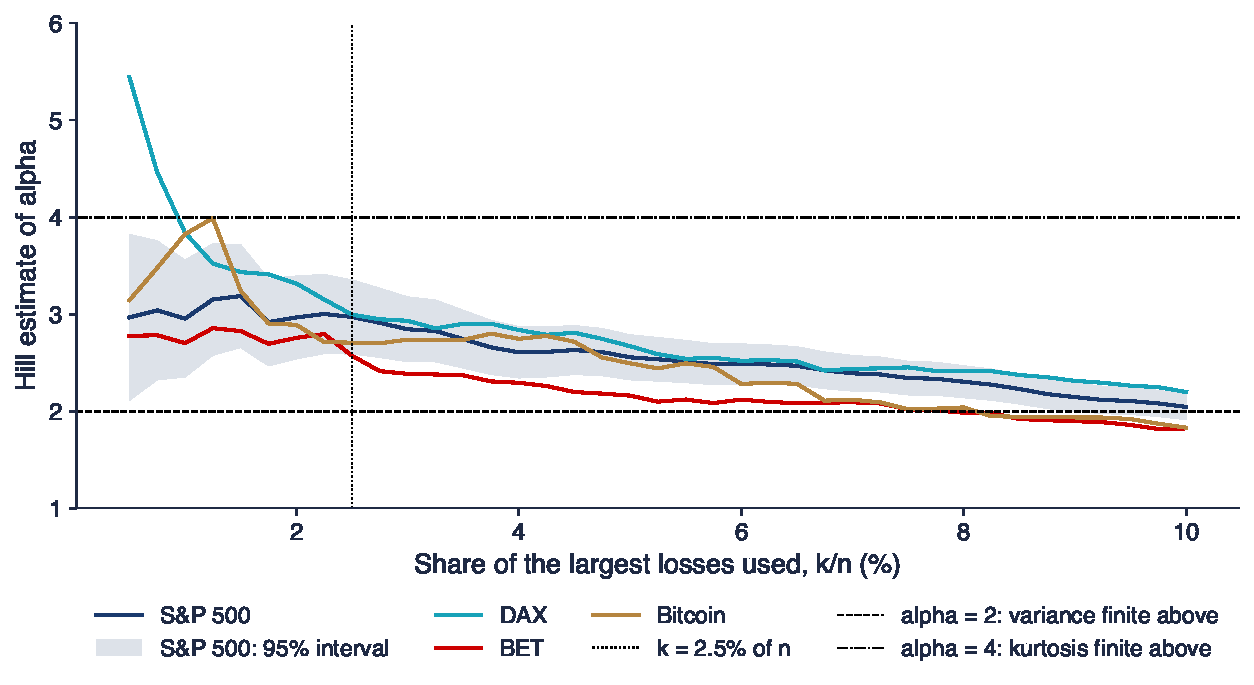
\includegraphics[width=0.97\textwidth,height=0.60\textheight,keepaspectratio]{sfm_ch5_hill_plot.pdf}
\end{center}
\vspace{-0.25cm}
\begin{itemize}
    \item Between 1\% and 5\% of $n$ the curves are fairly flat, mostly between 2 and 3.5; band: 95\% interval for the S\&P 500
    \item Beyond 5\% the estimates drift down: the body of the distribution biases $\hat\alpha$
\end{itemize}
\quantlet{SFM\_ch5\_hill}{\qlurl{SFM_ch5_hill}}
\end{frame}

\begin{frame}{Inference for the Hill Estimator}
\itemsize{\small}
\begin{itemize}
    \item For i.i.d.\ data with a Pareto-type tail: $\sqrt{k}\,(\hat\alpha_k - \alpha) \to N(0, \alpha^2)$, for $k \to \infty$, $k/n \to 0$
    \begin{itemize}
        \item i.i.d.: independent and identically distributed; $\mathrm{SE} = \hat\alpha/\sqrt{k}$, 95\% CI (confidence interval) $\hat\alpha(1 \pm 1.96/\sqrt{k})$
    \end{itemize}
    \item Returns are not independent: large losses come in clusters (volatility clustering)
    \begin{itemize}
        \item \textbf{moving-block bootstrap}: resample blocks of 20 consecutive days, recompute $\hat\alpha$, take the standard deviation
        \item the blocks keep the clusters together, so the standard error is honest about the dependence
    \end{itemize}
    \item Same rule for every series: $k = 2.5\%$ of $n$, 500 bootstrap samples
\end{itemize}
\end{frame}

\begin{frame}{Hill Estimates for Four Markets}
\itemsize{\footnotesize}
\begin{center}
\scriptsize
\begin{tabular}{lrrrrrrrr}
\toprule
& $n$ & $k$ & $\hat\alpha$ & 95\% CI & SE i.i.d. & SE block & $k = 1\%$ / $5\%$ & gains \\
\midrule
S\&P 500 & 9\,240 & 231 & $2.97$ & $[2.59, 3.35]$ & $0.20$ & $0.30$ & $2.95$ / $2.56$ & $2.96$ \\
DAX & 9\,288 & 232 & $3.00$ & $[2.61, 3.38]$ & $0.20$ & $0.20$ & $3.84$ / $2.67$ & $3.22$ \\
BET & 7\,243 & 181 & $2.57$ & $[2.20, 2.95]$ & $0.19$ & $0.23$ & $2.70$ / $2.16$ & $2.82$ \\
Bitcoin & 4\,384 & 109 & $2.71$ & $[2.20, 3.21]$ & $0.26$ & $0.23$ & $3.83$ / $2.49$ & $3.37$ \\
\bottomrule
\end{tabular}
\end{center}
\begin{itemize}
    \item Losses: $\hat\alpha$ between $2.57$ and $3.00$; the intervals exclude 2 (finite variance) and lie below 4 (no finite kurtosis)
    \item The block-bootstrap SE is close to the i.i.d.\ one here; the estimates move with $k$ by more than one SE
    \item Last column: the Hill index of gains ($r_t > 0$), same $k$
\end{itemize}\quantlet{SFM\_ch5\_hill}{\qlurl{SFM_ch5_hill}}
\end{frame}

\begin{frame}{From the Tail Index to a Quantile}
\itemsize{\small}
\begin{itemize}
    \item \textbf{Hill (Weissman) quantile} \refWeissman: $\hat x_p = L_{(k+1)}\Big(\dfrac{k}{n p}\Big)^{1/\hat\alpha}$
    \begin{itemize}
        \item the loss exceeded with probability $p$, extrapolated from the threshold with the power law; SFE Quantlet SFEhillquantile
    \end{itemize}
    \item \textbf{Worked example}, S\&P 500, VaR 0.1\%: $n = 9\,240$, $k = 231$, $L_{(k+1)} = 2.34\%$, $\hat\alpha = 2.97$
    \begin{itemize}
        \item $k/(np) = 231/9.24 = 25.0$; $25.0^{1/2.97} = 2.95$
        \item $\hat x_{0.001} = 2.34 \times 2.95 = 6.92\%$; empirical 0.1\% quantile: $6.94\%$
    \end{itemize}
    \item The extrapolation is only as good as $\hat\alpha$: an error of one SE in $\hat\alpha$ moves $\hat x_p$ noticeably
\end{itemize}\quantlet{SFM\_ch5\_hill}{\qlurl{SFM_ch5_hill}}
\end{frame}

\begin{frame}{Four Stocks of the Bucharest Stock Exchange}
\itemsize{\footnotesize}
\begin{columns}[T]
\begin{column}{0.60\textwidth}
\begin{center}
\scriptsize
\begin{tabular}{lrrrrr}
\toprule
& $n$ & $\hat\alpha$ & 95\% CI & SE block & gains \\
\midrule
OMV Petrom (SNP) & 3\,815 & $2.96$ & $[2.36, 3.56]$ & $0.39$ & $3.71$ \\
BRD & 3\,771 & $3.22$ & $[2.57, 3.87]$ & $0.33$ & $3.77$ \\
Banca Transilvania (TLV) & 3\,788 & $2.49$ & $[1.98, 2.99]$ & $0.28$ & $3.55$ \\
Transgaz (TGN) & 3\,725 & $3.02$ & $[2.41, 3.64]$ & $0.31$ & $3.56$ \\
\bottomrule
\end{tabular}
\end{center}
\begin{itemize}
    \item Daily log returns of the adjusted close since 2010, $k = 2.5\%$ of $n$
    \item TLV: the two days 30--31 May 2016 are removed, an adjustment applied one day late (\sfmchlink{https://danpele.github.io/SFM/EN/Courses/chapter2_classical_distributions_stylised_facts.pdf}{Chapter 2})
    \item All four: $\hat\alpha$ between $2.49$ and $3.22$, as for the indices; the losses have heavier tails than the gains
\end{itemize}
\end{column}
\begin{column}{0.36\textwidth}
\centering

\includegraphics[height=0.32\textheight]{ch5_bvb_palace_2019.jpg}\\[1mm]
\imgcap{The Stock Exchange Palace, Bucharest}
\imgcredit{https://commons.wikimedia.org/wiki/File:Stock_Exchange_Palace_(Bucharest).jpg}{Photo: Neoclassicism Enthusiast (2019); CC BY-SA 4.0; Wikimedia Commons}
\end{column}
\end{columns}\quantlet{SFM\_ch5\_hill}{\qlurl{SFM_ch5_hill}}
\end{frame}

\begin{frame}{Hill Plots of the BVB Stocks}
\itemsize{\footnotesize}
\begin{center}
    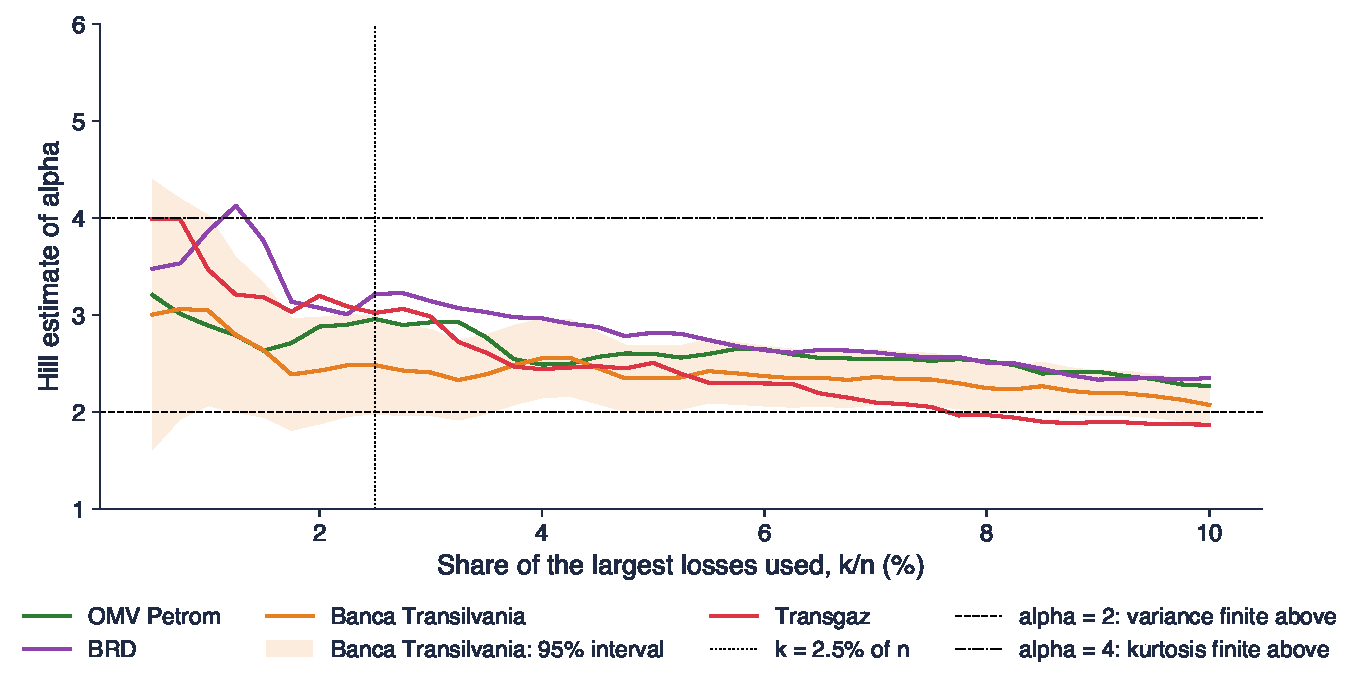
\includegraphics[width=0.97\textwidth,height=0.58\textheight,keepaspectratio]{sfm_ch5_hill_bvb.pdf}
\end{center}
\vspace{-0.25cm}
\begin{itemize}
    \item Shorter samples ($n \approx 3\,800$): wider bands (TLV shown) and more wiggles at small $k$
    \item No stock has $\hat\alpha$ below 2 in the flat region: variances are finite
\end{itemize}
\quantlet{SFM\_ch5\_hill}{\qlurl{SFM_ch5_hill}}
\end{frame}

\begin{frame}{Recap: The Hill Estimator}
\itemsize{\small}
\begin{itemize}
    \item $\hat\alpha_k = [\frac1k\sum_{i \le k}\ln(L_{(i)}/L_{(k+1)})]^{-1}$, the ML estimator of a Pareto tail
    \item Choose $k$ where the Hill plot is flat; fix the rule in advance
    \item SE $\approx \hat\alpha/\sqrt{k}$; block bootstrap for dependent returns
    \item Indices and BVB stocks: $\hat\alpha$ between $2.49$ and $3.22$, finite variance, infinite kurtosis
\end{itemize}
\end{frame}


%=============================================================================
\section{The Mean Excess Function}
%=============================================================================

\begin{frame}{The Mean Excess Function}
\itemsize{\small}
\begin{itemize}
    \item \textbf{Mean excess function}: $e(u) = E[L - u \mid L > u]$, the average loss beyond $u$, given that $u$ is exceeded
    \begin{itemize}
        \item empirical version: the average of $L_i - u$ over the losses with $L_i > u$
    \end{itemize}
    \item Its shape tells the type of tail
    \begin{itemize}
        \item Exponential: $e(u)$ constant (no memory)
        \item Pareto with $\alpha > 1$: $e(u) = u/(\alpha - 1)$, a rising straight line
        \item Normal: $e(u)$ falls towards 0 (roughly $1/u$ for a standard Normal)
    \end{itemize}
    \item \textbf{Example}: Pareto tail with $\alpha = 3$: $e(u) = u/2$
    \begin{itemize}
        \item beyond a 2\% loss the average extra loss is $1.0\%$; beyond 4\% it is $2.0\%$: the deeper, the worse
    \end{itemize}
\end{itemize}
\end{frame}

\begin{frame}{Empirical Mean Excess of Daily Losses}
\itemsize{\footnotesize}
\begin{center}
    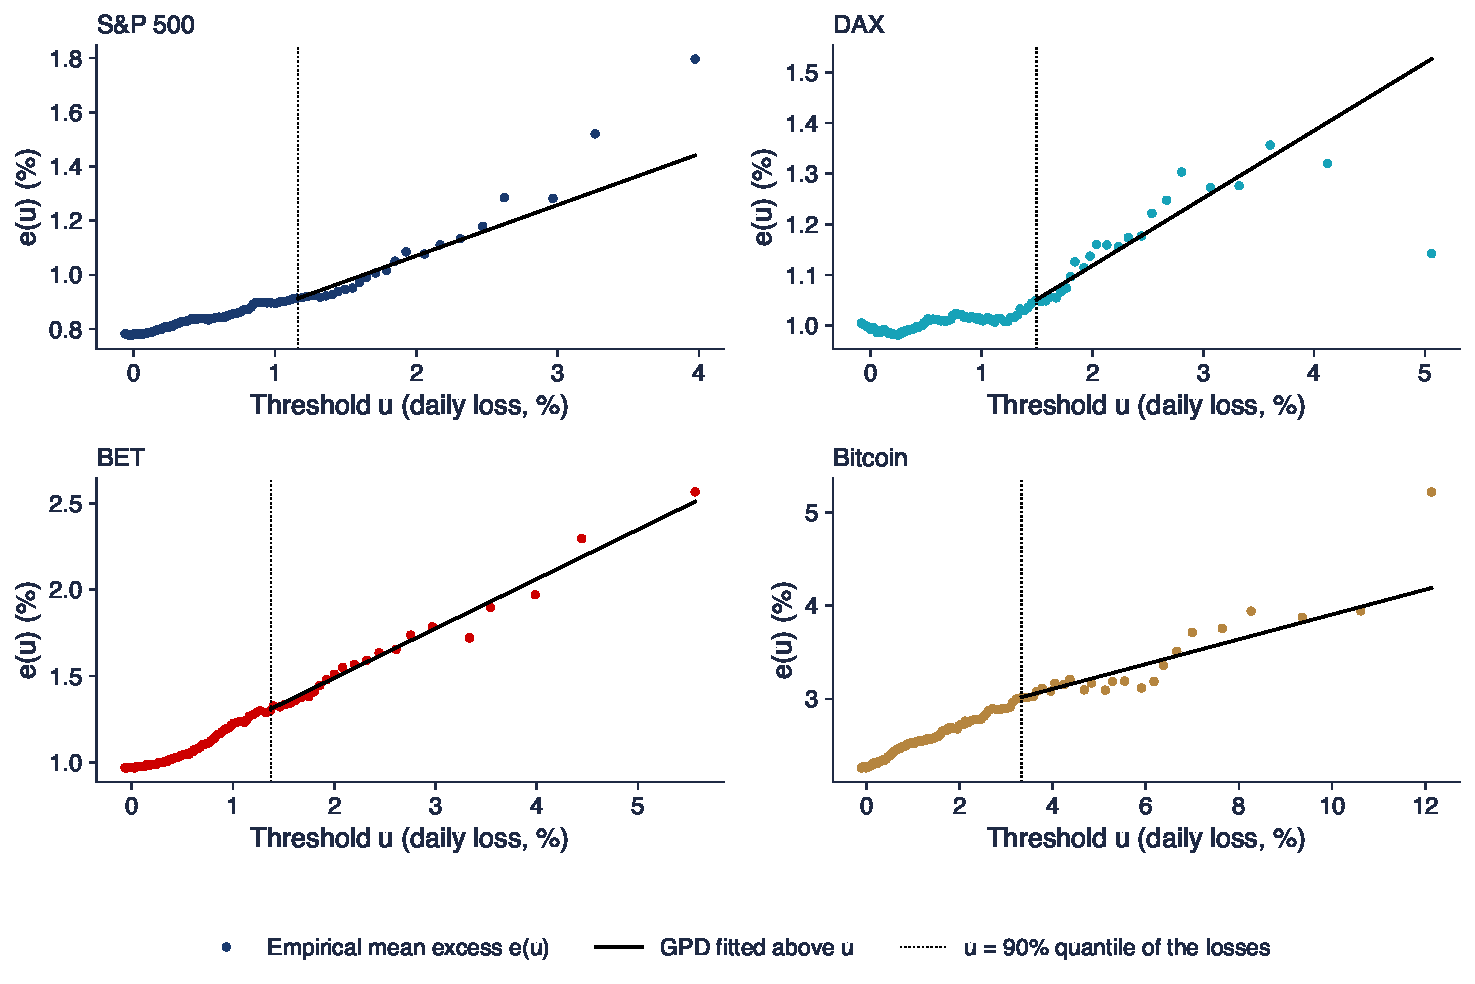
\includegraphics[width=0.97\textwidth,height=0.62\textheight,keepaspectratio]{sfm_ch5_mean_excess.pdf}
\end{center}
\vspace{-0.25cm}
\begin{itemize}
    \item All four functions rise above the 90\% quantile $u$ (dotted): a heavy, Pareto-type tail; black: the line implied by the GPD fitted above $u$
    \item The last points rest on very few losses and jump around: do not read them literally
\end{itemize}
\quantlet{SFM\_ch5\_mean\_excess}{\qlurl{SFM_ch5_mean_excess}}
\end{frame}

\begin{frame}{Reading the Mean Excess Plot}
\itemsize{\small}
\begin{itemize}
    \item Look for the threshold above which $e(u)$ becomes roughly a straight line
    \begin{itemize}
        \item a rising line means a heavy tail; its slope gives a first guess of the shape of the tail
    \end{itemize}
    \item At the 90\% quantile: $e(u)$ is $0.92\%$ for the S\&P 500 ($u = 1.16\%$) and $1.30\%$ for the BET ($u = 1.38\%$)
    \begin{itemize}
        \item on a day with a loss above $u$, the loss beyond $u$ is about as large as $u$ itself
    \end{itemize}
    \item The mean excess function is one of the tools for choosing the threshold of the peaks over threshold method (Section 6)
    \item Ported from the SFE Quantlet SFEMeanExcessFun
\end{itemize}\quantlet{SFM\_ch5\_mean\_excess}{\qlurl{SFM_ch5_mean_excess}}
\end{frame}


%=============================================================================
\section{Block Maxima and the GEV Distribution}
%=============================================================================

\begin{frame}{Block Maxima}
\itemsize{\small}
\begin{columns}[T]
\begin{column}{0.62\textwidth}
\begin{itemize}
    \item Split the losses into blocks of equal length and keep the largest loss of each block
    \begin{itemize}
        \item $M_n = \max(L_1, \dots, L_n)$, here the largest daily loss of each calendar month ($n \approx 21$)
    \end{itemize}
    \item Question: what is the law of $M_n$ for large $n$?
    \begin{itemize}
        \item the analogue of the central limit theorem, for maxima instead of sums
    \end{itemize}
    \item \refFT\ found the three possible limit laws, studying the largest of a sample
\end{itemize}
\end{column}
\begin{column}{0.34\textwidth}
\centering

\includegraphics[height=0.42\textheight]{ch5_fisher_1913.jpg}\\[1mm]
\imgcap{Ronald A. Fisher (1890--1962), in 1913}
\imgcredit{https://commons.wikimedia.org/wiki/File:Youngronaldfisher2.JPG}{Photo: unknown author (1913); public domain; Wikimedia Commons}
\end{column}
\end{columns}
\end{frame}

\begin{frame}{The Fisher--Tippett--Gnedenko Theorem}
\itemsize{\small}
\begin{itemize}
    \item $L_1, L_2, \dots$ i.i.d. If there are constants $a_n > 0$, $b_n$ such that $P\Big(\dfrac{M_n - b_n}{a_n} \le x\Big) \to H(x)$, non-degenerate,
    \begin{itemize}
        \item then $H$ is a \textbf{GEV} (generalised extreme value) distribution \refFT, \refGnedenko
    \end{itemize}
    \item \textbf{GEV} with shape $\xi$, location $\mu$, scale $\sigma > 0$ (the unified form of \refJenkinson)
    \begin{itemize}
        \item $H(x) = \exp\Big\{-\Big[1 + \xi\,\dfrac{x - \mu}{\sigma}\Big]^{-1/\xi}\Big\}$ for $1 + \xi(x - \mu)/\sigma > 0$
        \item $\xi = 0$: $H(x) = \exp\{-e^{-(x - \mu)/\sigma}\}$, the limit as $\xi \to 0$
    \end{itemize}
    \item Whatever the law of the losses, the normalised maximum has only one family of possible limits
\end{itemize}
\end{frame}

\begin{frame}{Three Types in One Family}
\itemsize{\small}
\begin{columns}[T]
\begin{column}{0.64\textwidth}
\begin{itemize}
    \item \textbf{Fréchet} ($\xi > 0$): heavy tail, $1 - H(x) \sim x^{-1/\xi}$
    \begin{itemize}
        \item tail index $\alpha = 1/\xi$; the case of financial losses
    \end{itemize}
    \item \textbf{Gumbel} ($\xi = 0$): light, exponential tail
    \begin{itemize}
        \item maxima of Normal, lognormal and Exponential variables
    \end{itemize}
    \item \textbf{Weibull} ($\xi < 0$): a finite upper end point $\mu - \sigma/\xi$
    \begin{itemize}
        \item maxima of bounded variables (Uniform, Beta)
    \end{itemize}
    \item The set of laws whose maxima converge to a given $H$ is its \textbf{maximum domain of attraction}
\end{itemize}
\end{column}
\begin{column}{0.32\textwidth}
\centering
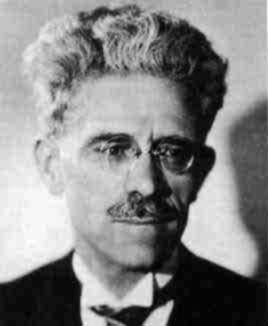
\includegraphics[height=0.40\textheight]{ch5_frechet.jpg}\\[1mm]
\imgcap{Maurice Fréchet (1878--1973)}
\imgcredit{https://commons.wikimedia.org/wiki/File:Frechet.jpeg}{Photo: unknown author; public domain; Wikimedia Commons}
\end{column}
\end{columns}
\end{frame}

\begin{frame}{The Three Extreme Value Laws}
\itemsize{\footnotesize}
\begin{center}
    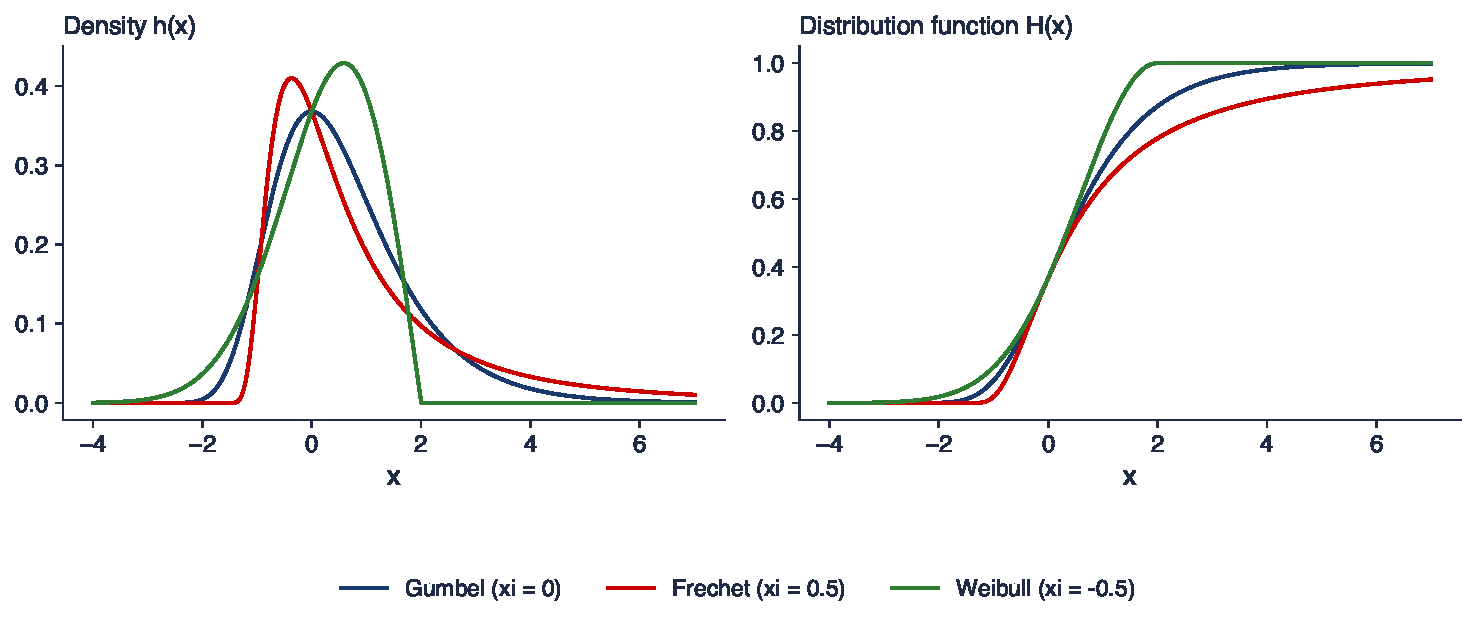
\includegraphics[width=0.97\textwidth,height=0.56\textheight,keepaspectratio]{sfm_ch5_gev_types.pdf}
\end{center}
\vspace{-0.25cm}
\begin{itemize}
    \item Standard location and scale ($\mu = 0$, $\sigma = 1$): Fréchet has the longest right tail, Weibull stops at $x = 2$
    \item Ported from the SFE Quantlet SFEevt1
\end{itemize}
\quantlet{SFM\_ch5\_gev\_block\_maxima}{\qlurl{SFM_ch5_gev_block_maxima}}
\end{frame}

\begin{frame}{The Theorem in a Simulation}
\itemsize{\footnotesize}
\begin{center}
    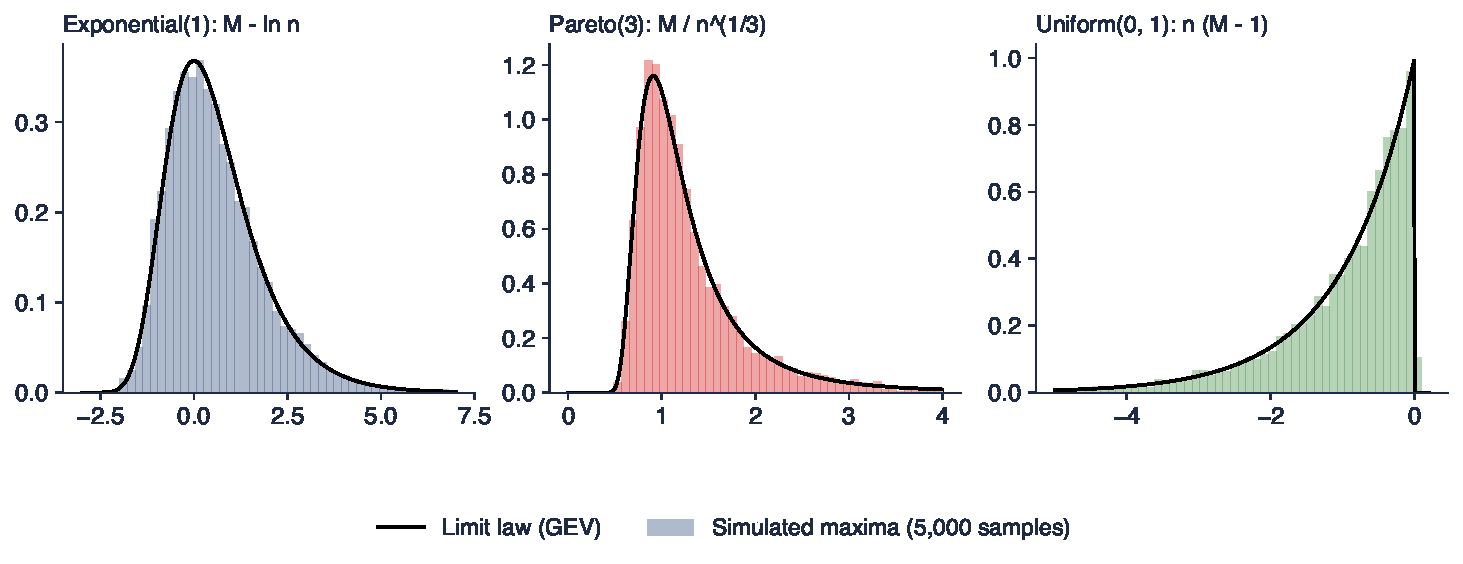
\includegraphics[width=0.97\textwidth,height=0.44\textheight,keepaspectratio]{sfm_ch5_maxima_sim.pdf}
\end{center}
\vspace{-0.25cm}
\begin{itemize}
    \item 5,000 samples of $n = 250$; Exponential maxima minus $\ln n$ $\to$ Gumbel; Pareto(3) maxima over $n^{1/3}$ $\to$ Fréchet with $\xi = 1/3$; Uniform: $n(M_n - 1)$ $\to$ Weibull
    \item \textbf{Question for the room}: daily losses have a tail index near 3; which type do their monthly maxima follow?
    \item \textbf{Answer}: Fréchet, with $\xi = 1/\alpha \approx 0.3$
\end{itemize}
\quantlet{SFM\_ch5\_gev\_block\_maxima}{\qlurl{SFM_ch5_gev_block_maxima}}
\end{frame}

\begin{frame}{GEV Fits to Monthly Maxima}
\itemsize{\footnotesize}
\begin{center}
\footnotesize
\begin{tabular}{lrrrrrr}
\toprule
& months & $\hat\xi$ & 95\% CI & $\hat\mu$ (\%) & $\hat\sigma$ (\%) & $1/\hat\xi$ \\
\midrule
S\&P 500 & 440 & $0.21$ & $[0.13, 0.29]$ & $1.31$ & $0.74$ & $4.7$ \\
DAX & 440 & $0.17$ & $[0.09, 0.25]$ & $1.69$ & $0.91$ & $5.9$ \\
BET & 342 & $0.36$ & $[0.26, 0.46]$ & $1.47$ & $0.92$ & $2.7$ \\
Bitcoin & 144 & $0.23$ & $[0.08, 0.38]$ & $5.19$ & $2.85$ & $4.3$ \\
\bottomrule
\end{tabular}
\end{center}
\begin{itemize}
    \item Maximum likelihood on the monthly maxima of daily losses; SE from the curvature of the log-likelihood
    \item $\hat\xi > 0$ for all four series: Fréchet type, heavy tails; the intervals exclude 0 (Gumbel)
    \item $1/\hat\xi$ is a second estimate of the tail index; with only one loss per month it is less precise than Hill
\end{itemize}\quantlet{SFM\_ch5\_gev\_block\_maxima}{\qlurl{SFM_ch5_gev_block_maxima}}
\end{frame}

\begin{frame}{Does the GEV Fit? PP and QQ Plots}
\itemsize{\footnotesize}
\begin{center}
    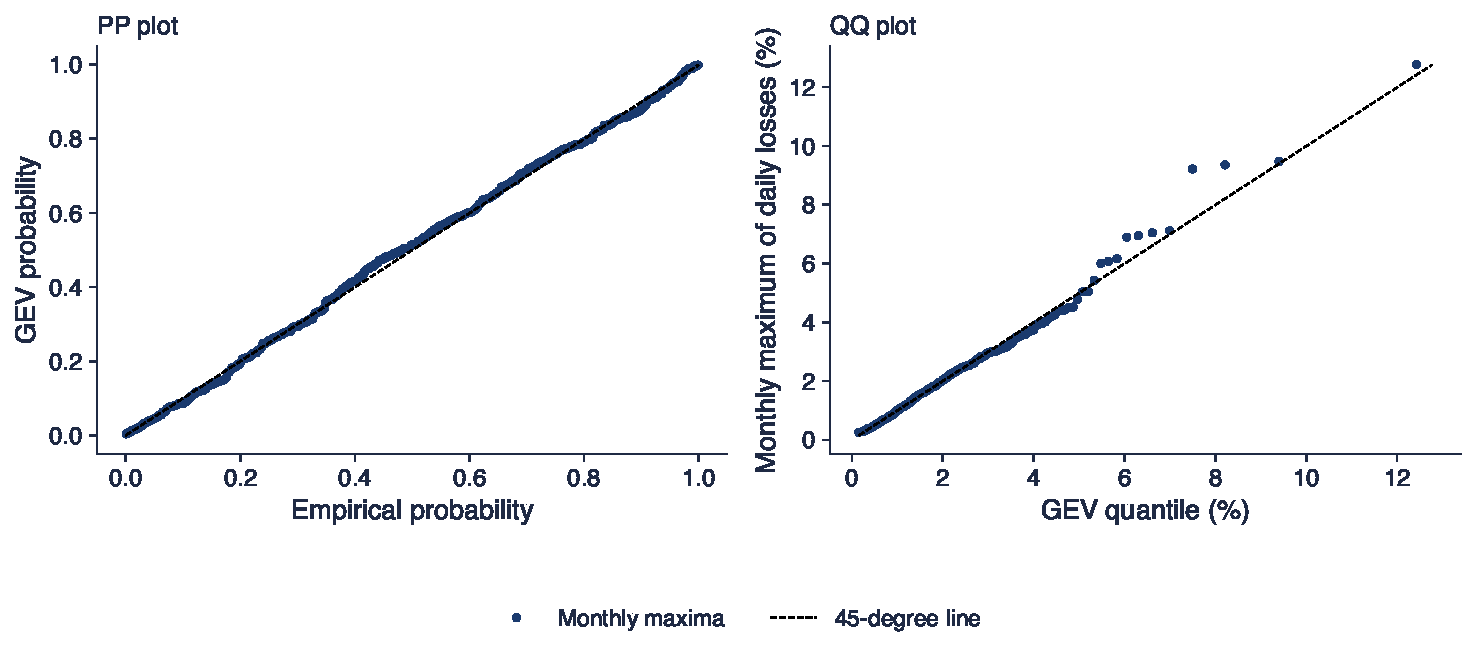
\includegraphics[width=0.97\textwidth,height=0.54\textheight,keepaspectratio]{sfm_ch5_gev_ppqq.pdf}
\end{center}
\vspace{-0.25cm}
\begin{itemize}
    \item \textbf{PP plot}: fitted probability $H(m_{(i)})$ against the empirical $(i - 0.5)/n$; \textbf{QQ plot}: observed maxima against fitted quantiles; S\&P 500
    \item Both close to the 45-degree line; the QQ plot shows the few largest months (2008, 2020) a little above: the hardest part to fit
\end{itemize}
\quantlet{SFM\_ch5\_gev\_block\_maxima}{\qlurl{SFM_ch5_gev_block_maxima}}
\end{frame}

\begin{frame}{Return Levels}
\itemsize{\small}
\begin{itemize}
    \item \textbf{Return level} for a return period of $T$ years: the level that the monthly maximum exceeds on average once every $T$ years
    \begin{itemize}
        \item $z_T = H^{-1}(1 - 1/m)$ with $m = 12T$ months: $z_T = \mu + \dfrac{\sigma}{\xi}\big[(-\ln(1 - 1/m))^{-\xi} - 1\big]$
    \end{itemize}
    \item \textbf{Worked example}, S\&P 500, $T = 10$ years: $\hat\xi = 0.211$, $\hat\mu = 1.311$, $\hat\sigma = 0.737$
    \begin{itemize}
        \item $m = 120$; $-\ln(1 - 1/120) = 0.00837$; raised to $-\hat\xi$: $2.747$
        \item $z_{10} = 1.311 + (0.737/0.211)(2.747 - 1) = 7.4\%$
    \end{itemize}
    \item A daily loss of about $7.4\%$ in the S\&P 500 is a ``10-year event''; it was exceeded in 4 months of 36.7 years
\end{itemize}
\end{frame}

\begin{frame}{Return Level Plot}
\itemsize{\footnotesize}
\begin{center}
    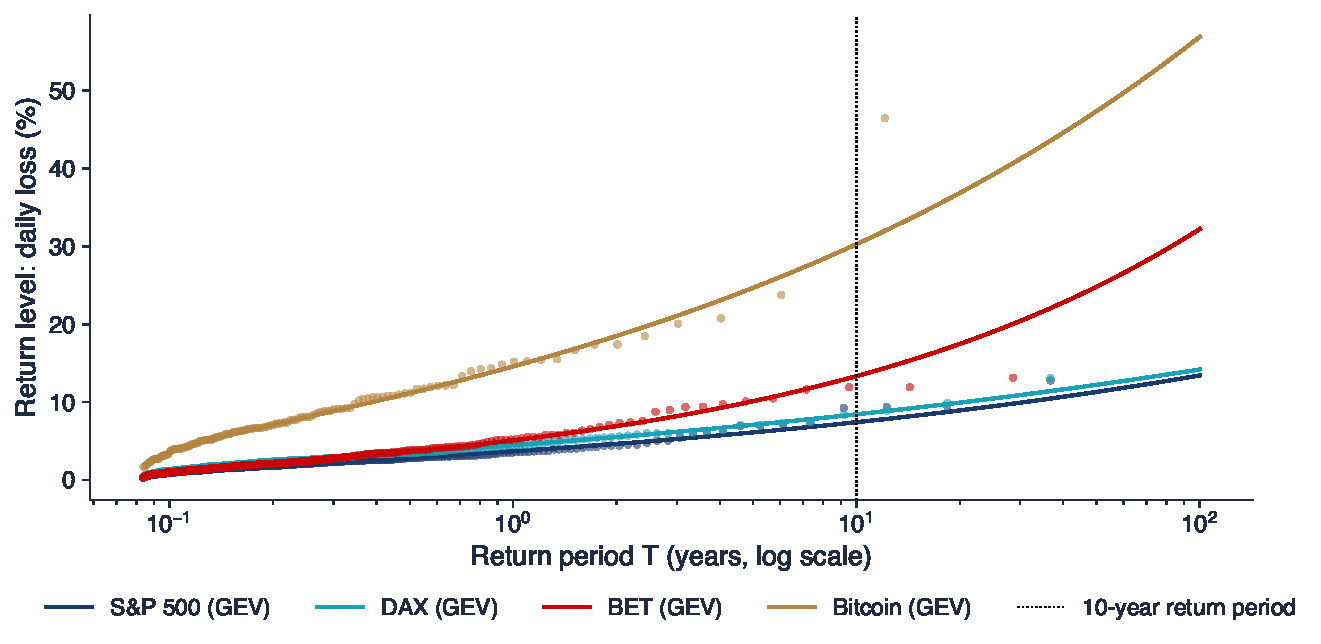
\includegraphics[width=0.97\textwidth,height=0.58\textheight,keepaspectratio]{sfm_ch5_return_levels.pdf}
\end{center}
\vspace{-0.25cm}
\begin{itemize}
    \item Lines: GEV return levels; dots: observed monthly maxima at their empirical return periods
    \item Beyond the length of the sample (36.7 years for the S\&P 500, 12 for Bitcoin) the curves are extrapolation
\end{itemize}
\quantlet{SFM\_ch5\_gev\_block\_maxima}{\qlurl{SFM_ch5_gev_block_maxima}}
\end{frame}

\begin{frame}{How Large Is a 10-Year Loss?}
\itemsize{\footnotesize}
\begin{center}
\footnotesize
\begin{tabular}{lrrrrrr}
\toprule
& 1 year & 10 years & 95\% interval & 50 years & largest observed & years of data \\
\midrule
S\&P 500 & $3.7$ & $7.4$ & $[6.2, 8.9]$ & $11.3$ & $12.8$ & $36.7$ \\
DAX & $4.5$ & $8.4$ & $[7.1, 9.9]$ & $12.2$ & $13.1$ & $36.7$ \\
BET & $5.1$ & $13.3$ & $[10.3, 17.5]$ & $24.8$ & $13.1$ & $28.5$ \\
Bitcoin & $14.6$ & $30.3$ & $[21.2, 41.1]$ & $47.4$ & $46.5$ & $12$ \\
\bottomrule
\end{tabular}
\end{center}
\begin{itemize}
    \item Daily loss (\%) exceeded on average once in $T$ years; interval: bootstrap of the monthly maxima (200 samples)
    \item BET: $\hat\xi = 0.36$ makes the 50-year level $24.8\%$, almost twice the largest loss seen: a small change in $\hat\xi$, a large change far out
    \item Block maxima use one loss per month: the peaks over threshold method uses all large losses
\end{itemize}\quantlet{SFM\_ch5\_gev\_block\_maxima}{\qlurl{SFM_ch5_gev_block_maxima}}
\end{frame}

\begin{frame}{Recap: Block Maxima}
\itemsize{\small}
\begin{itemize}
    \item Maxima of i.i.d.\ variables can only converge to a GEV law (Fisher--Tippett--Gnedenko)
    \item $\xi > 0$ Fréchet (heavy, $\alpha = 1/\xi$), $\xi = 0$ Gumbel, $\xi < 0$ Weibull
    \item Monthly maxima of daily losses: Fréchet, $\hat\xi$ between $0.17$ and $0.36$
    \item Return level: the loss exceeded once in $T$ years; far beyond the sample it is extrapolation
\end{itemize}
\end{frame}


%=============================================================================
\section{Peaks over Threshold and the GPD}
%=============================================================================

\begin{frame}{Peaks over Threshold}
\itemsize{\small}
\begin{columns}[T]
\begin{column}{0.58\textwidth}
\begin{itemize}
    \item \textbf{POT} (peaks over threshold): fix a high threshold $u$ and keep every loss above it
    \begin{itemize}
        \item the \textbf{excess} over $u$: $Y = L - u$, given $L > u$
        \item excess distribution: $F_u(y) = P(L - u \le y \mid L > u)$
    \end{itemize}
    \item Uses all large losses, not one per block: more data in the tail
    \item The method behind most EVT estimates of VaR and ES \refMF, \refQRM
\end{itemize}
\end{column}
\begin{column}{0.38\textwidth}
\centering

\includegraphics[height=0.36\textheight]{ch5_dehaan_1987.jpg}\\[1mm]
\imgcap{Laurens de Haan, Oberwolfach, 1987}
\imgcredit{https://commons.wikimedia.org/wiki/File:Laurens_de_haan.jpg}{Photo: Konrad Jacobs (1987), Oberwolfach Photo Collection; CC BY-SA 2.0 de; Wikimedia Commons}
\end{column}
\end{columns}
\end{frame}

\begin{frame}{The Pickands--Balkema--de Haan Theorem}
\itemsize{\small}
\begin{itemize}
    \item If the maxima of $L$ converge to a GEV with shape $\xi$, then for high thresholds
    \begin{itemize}
        \item $F_u(y) \approx G_{\xi, \beta(u)}(y)$, the \textbf{GPD} (generalised Pareto distribution) \refPickands, \refBdH
    \end{itemize}
    \item $G_{\xi, \beta}(y) = 1 - \Big(1 + \xi\,\dfrac{y}{\beta}\Big)^{-1/\xi}$, $y \ge 0$ (for $\xi < 0$: $y \le -\beta/\xi$); $\xi = 0$: $1 - e^{-y/\beta}$
    \begin{itemize}
        \item shape $\xi$: the \textbf{same} as in the GEV; scale $\beta > 0$ depends on $u$
        \item $\xi > 0$: Pareto-type tail with $\alpha = 1/\xi$; $\xi = 0$: Exponential; $\xi < 0$: bounded
    \end{itemize}
    \item Moments of the GPD: mean $\beta/(1 - \xi)$ if $\xi < 1$; variance finite if $\xi < 1/2$
    \begin{itemize}
        \item mean excess of a GPD: $e(v) = \dfrac{\beta + \xi(v - u)}{1 - \xi}$, a straight line in $v > u$, as seen in Section 4
    \end{itemize}
\end{itemize}
\end{frame}

\begin{frame}{GPD Densities and Tails}
\itemsize{\footnotesize}
\begin{center}
    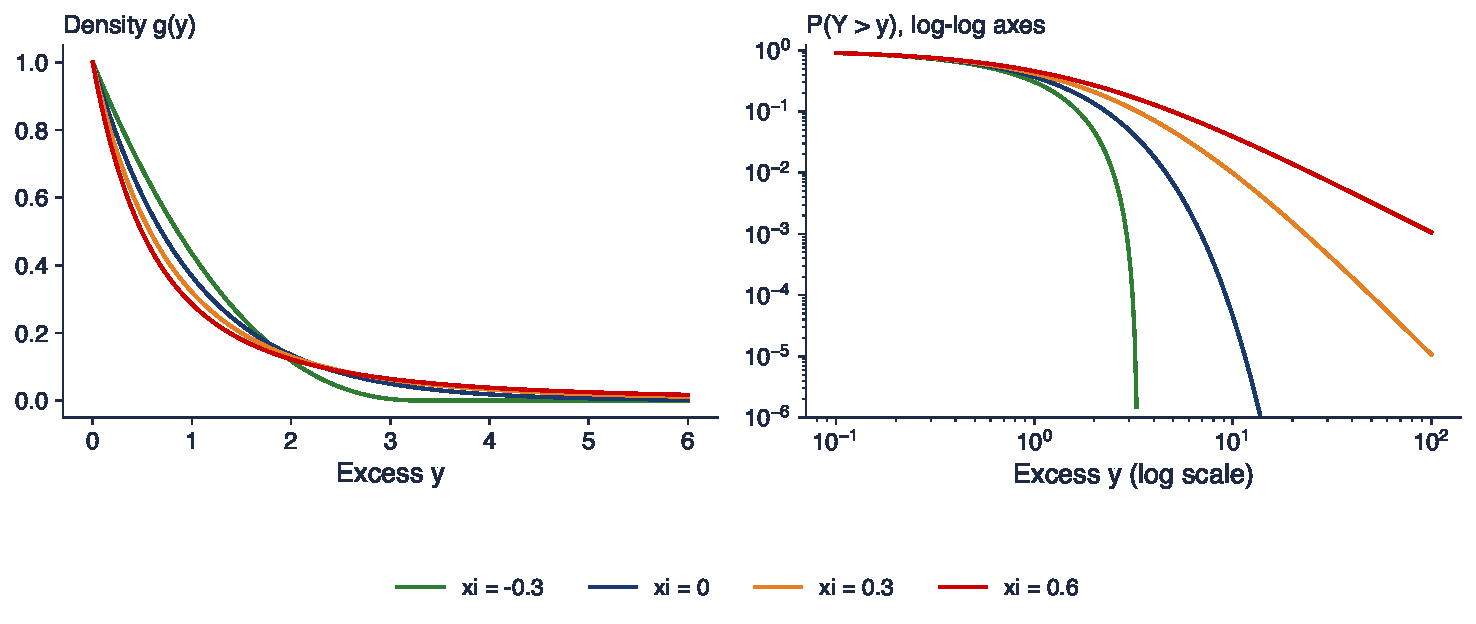
\includegraphics[width=0.97\textwidth,height=0.56\textheight,keepaspectratio]{sfm_ch5_gpd_densities.pdf}
\end{center}
\vspace{-0.25cm}
\begin{itemize}
    \item $\beta = 1$; the densities look alike near 0, the tails do not: on log-log axes only $\xi > 0$ gives straight lines
    \item $\xi = 0.3$ corresponds to a tail index $\alpha \approx 3.3$, close to stock returns
\end{itemize}
\quantlet{SFM\_ch5\_pot\_gpd}{\qlurl{SFM_ch5_pot_gpd}}
\end{frame}

\begin{frame}{Choosing the Threshold}
\itemsize{\small}
\begin{itemize}
    \item The same trade-off as $k$ in the Hill estimator
    \begin{itemize}
        \item $u$ too low: the GPD approximation is poor (bias); $u$ too high: few excesses (variance)
    \end{itemize}
    \item Graphical tools
    \begin{itemize}
        \item mean excess plot: roughly linear above $u$
        \item parameter stability plot: $\hat\xi$ should not change much when $u$ is raised further
    \end{itemize}
    \item Rule used here: $u =$ the 90\% quantile of the losses, i.e.\ the 10\% largest losses
    \begin{itemize}
        \item \refMF\ use $k = 100$ excesses in windows of $n = 1000$ days, the same share
        \item for the S\&P 500: $u = 1.16\%$ and $N_u = 924$ excesses
    \end{itemize}
\end{itemize}
\end{frame}

\begin{frame}{Parameter Stability}
\itemsize{\footnotesize}
\begin{center}
    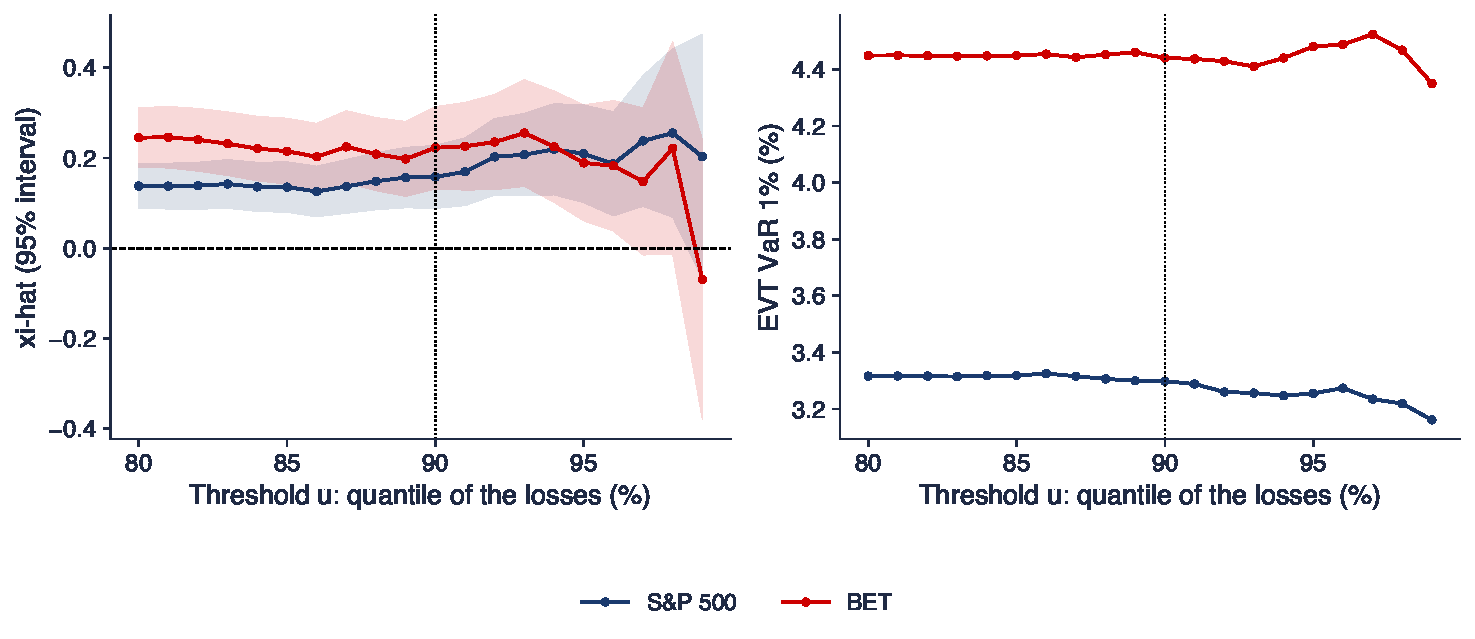
\includegraphics[width=0.97\textwidth,height=0.54\textheight,keepaspectratio]{sfm_ch5_threshold_stability.pdf}
\end{center}
\vspace{-0.25cm}
\begin{itemize}
    \item Left: $\hat\xi$ with 95\% interval for $u$ from the 80\% to the 99\% quantile; right: the EVT VaR 1\% for the same thresholds
    \item Between the 85\% and 95\% quantiles: S\&P 500 $\hat\xi \in [0.13, 0.22]$, VaR 1\% $\in [3.25, 3.33]\%$; the VaR barely moves
\end{itemize}
\quantlet{SFM\_ch5\_pot\_gpd}{\qlurl{SFM_ch5_pot_gpd}}
\end{frame}

\begin{frame}{GPD Fits above the 90\% Quantile}
\itemsize{\footnotesize}
\begin{center}
\footnotesize
\begin{tabular}{lrrrrrrr}
\toprule
& $n$ & $u$ (\%) & $N_u$ & $\hat\xi$ & SE & $\hat\beta$ & $1/\hat\xi$ \\
\midrule
S\&P 500 & 9\,240 & $1.16$ & 924 & $0.16$ & $0.04$ & $0.769$ & $6.3$ \\
DAX & 9\,288 & $1.50$ & 929 & $0.12$ & $0.04$ & $0.927$ & $8.5$ \\
BET & 7\,243 & $1.38$ & 725 & $0.22$ & $0.05$ & $1.018$ & $4.5$ \\
Bitcoin & 4\,384 & $3.33$ & 439 & $0.12$ & $0.05$ & $2.663$ & $8.5$ \\
\bottomrule
\end{tabular}
\end{center}
\begin{itemize}
    \item Maximum likelihood on the excesses $L - u$ \refDS; SE from the curvature of the log-likelihood
    \item $\hat\xi$ between $0.12$ and $0.22$: heavy tails with a finite variance ($\xi < 0.5$) for all four
    \item $1/\hat\xi$ is larger than the Hill $\hat\alpha$ (2.5\% of the losses): above the 90\% quantile, a GPD with a free scale $\beta$ needs a smaller $\xi$; the tail index is hard to pin down, so report more than one estimator
\end{itemize}\quantlet{SFM\_ch5\_pot\_gpd}{\qlurl{SFM_ch5_pot_gpd}}
\end{frame}

\begin{frame}{Does the GPD Fit? PP and QQ Plots}
\itemsize{\footnotesize}
\begin{center}
    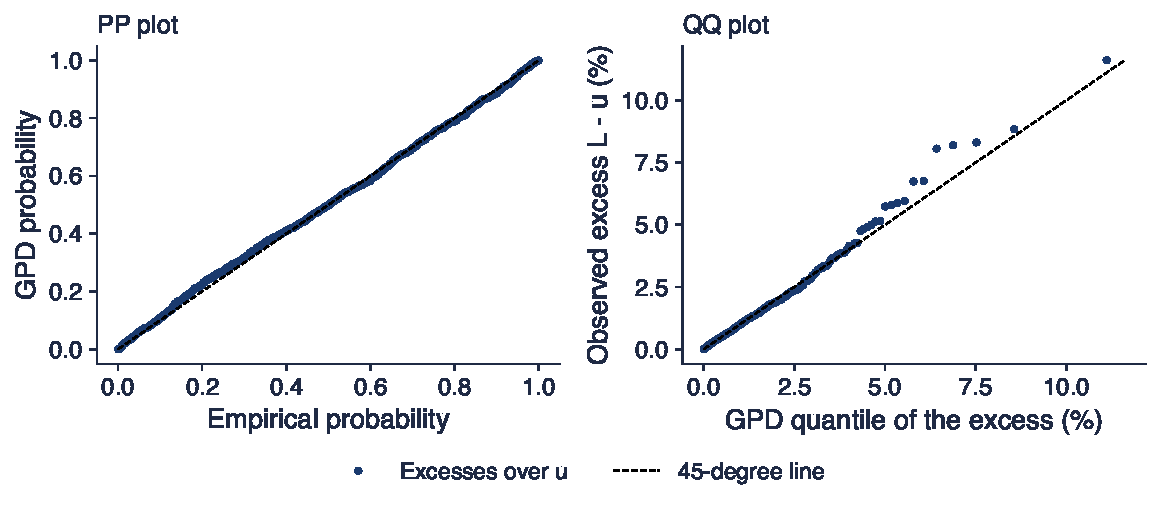
\includegraphics[width=0.97\textwidth,height=0.54\textheight,keepaspectratio]{sfm_ch5_gpd_ppqq.pdf}
\end{center}
\vspace{-0.25cm}
\begin{itemize}
    \item S\&P 500 excesses over $u$: the PP plot is on the line; the QQ plot is on the line up to excesses of about 4\%
    \item The largest excess ($11.6\%$, March 2020) against a fitted quantile of $11.1\%$; ported from the SFE Quantlets SFEtailGPareto\_pp and \_qq
\end{itemize}
\quantlet{SFM\_ch5\_pot\_gpd}{\qlurl{SFM_ch5_pot_gpd}}
\end{frame}

\begin{frame}{From the GPD to the Tail of the Losses}
\itemsize{\small}
\begin{itemize}
    \item For $x > u$: $P(L > x) = P(L > u)\,P(L > x \mid L > u)$
    \begin{itemize}
        \item estimate $P(L > u)$ by $N_u/n$ and $P(L > x \mid L > u)$ by the GPD
    \end{itemize}
    \item \textbf{Tail estimator}: $\hat{\bar F}(x) = \dfrac{N_u}{n}\Big(1 + \hat\xi\,\dfrac{x - u}{\hat\beta}\Big)^{-1/\hat\xi}$, $x > u$
    \item Historical data inside the sample, a fitted power law beyond it
    \begin{itemize}
        \item the model is used only where it is justified: above $u$
    \end{itemize}
    \item Inverting $\hat{\bar F}(x) = p$ gives VaR; integrating beyond it gives ES (Section 7)
\end{itemize}
\end{frame}

\begin{frame}{The Fitted Tails}
\itemsize{\footnotesize}
\begin{center}
    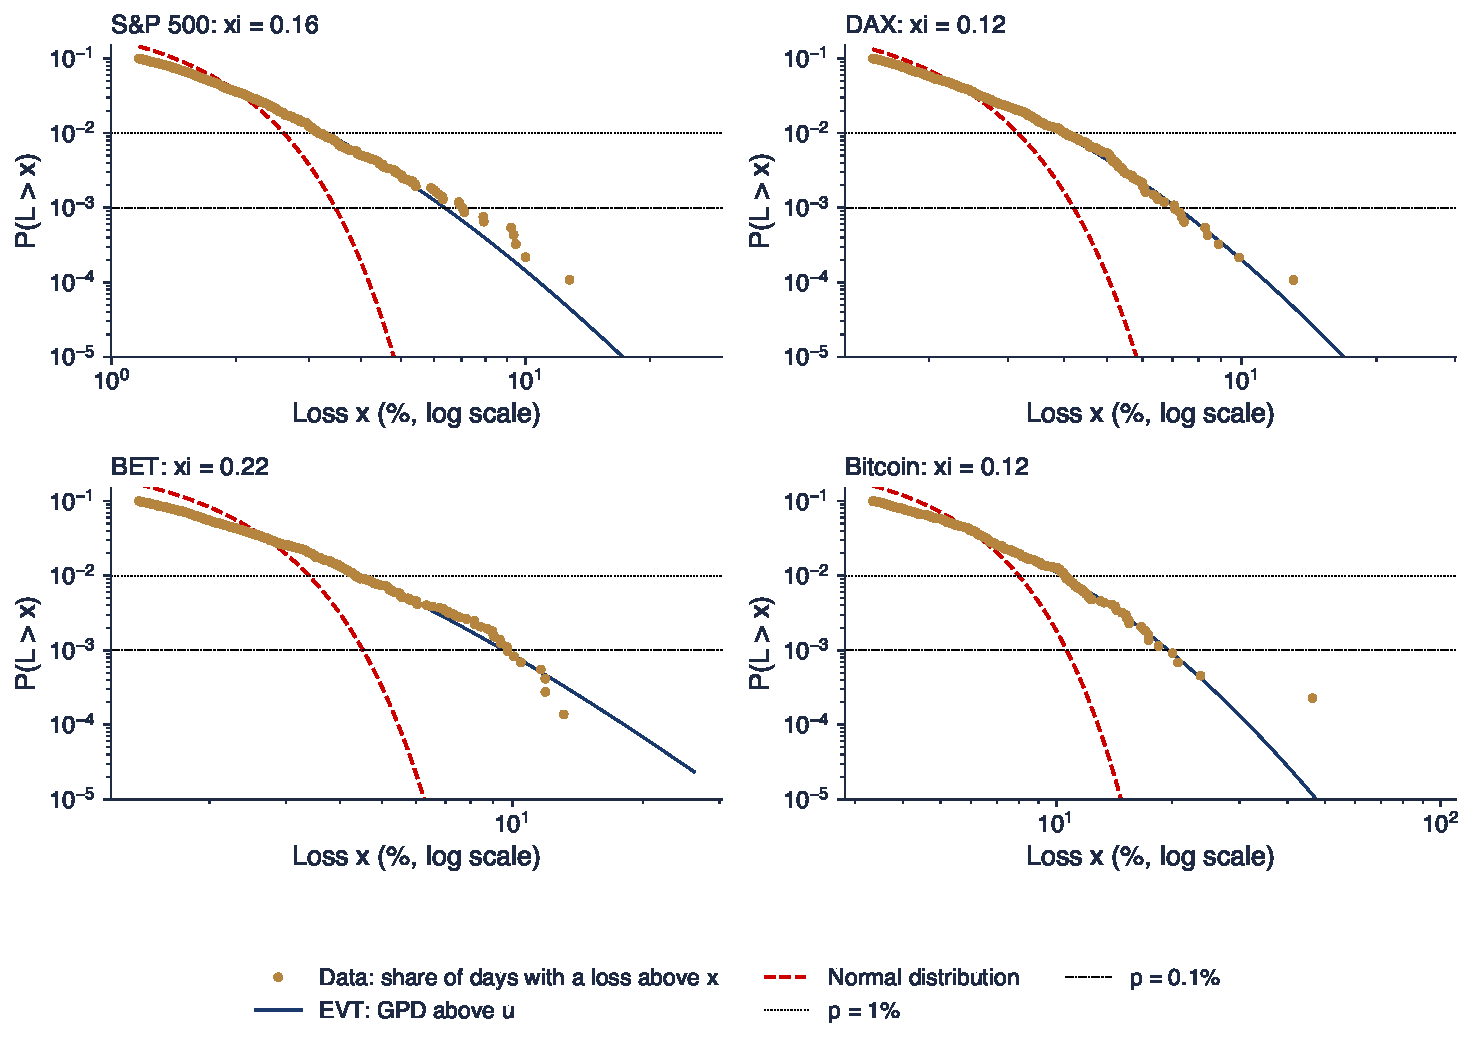
\includegraphics[width=0.97\textwidth,height=0.66\textheight,keepaspectratio]{sfm_ch5_tail_fit.pdf}
\end{center}
\vspace{-0.25cm}
\begin{itemize}
    \item Dots: share of days with a loss above $x$ (above $u$); blue: EVT tail estimator; red: Normal; dotted lines at $p = 1\%$ and $0.1\%$
    \item The GPD follows the data down to $10^{-4}$; the Normal tail leaves them before $p = 1\%$
\end{itemize}
\quantlet{SFM\_ch5\_pot\_gpd}{\qlurl{SFM_ch5_pot_gpd}}
\end{frame}

\begin{frame}{Back to the Crashes: How Often?}
\itemsize{\footnotesize}
\begin{center}
\footnotesize
\begin{tabular}{llrrr}
\toprule
& day & loss (\%) & Normal: once in (years) & EVT: once in (years) \\
\midrule
S\&P 500 & 16 March 2020 & ${-12.8}$ & $10^{27}$ & $89$ \\
DAX & 12 March 2020 & ${-13.1}$ & $10^{19}$ & $85$ \\
BET & 7 January 2009 & ${-13.1}$ & $10^{16}$ & $12$ \\
Bitcoin & 12 March 2020 & ${-46.5}$ & $10^{38}$ & $237$ \\
S\&P 500, Black Monday & 19 October 1987 & $-22.3$ & $10^{84}$ & $1\,600$ \\
\bottomrule
\end{tabular}
\end{center}
\begin{itemize}
    \item EVT waiting time: $1/(\hat{\bar F}(x) \times 252)$ years (365 for Bitcoin), with the POT fit of the whole sample
    \item EVT makes the COVID-19 days rare but plausible events of a lifetime; the Normal law makes them impossible
    \item 1987 is outside our data: EVT extrapolates it to a waiting time of about 1\,600 years, with a wide uncertainty
\end{itemize}\quantlet{SFM\_ch5\_pot\_gpd}{\qlurl{SFM_ch5_pot_gpd}}
\end{frame}

\begin{frame}{Recap: Peaks over Threshold}
\itemsize{\small}
\begin{itemize}
    \item Excesses over a high threshold follow approximately a GPD (Pickands--Balkema--de Haan)
    \item Same shape $\xi$ as the GEV; $\xi > 0$: power tail with $\alpha = 1/\xi$
    \item Threshold: mean excess and parameter stability; here the 90\% quantile
    \item Tail estimator: data up to $u$, GPD beyond; check with PP and QQ plots
\end{itemize}
\end{frame}


%=============================================================================
\section{VaR and ES by Extreme Value Theory}
%=============================================================================

\begin{frame}{VaR and ES: Definitions}
\itemsize{\small}
\begin{itemize}
    \item Losses $L = -r$ with distribution function $F_L$; level $p$ (e.g.\ $p = 1\%$)
    \begin{itemize}
        \item $\mathrm{VaR}_p = F_L^{-1}(1 - p) = -q_p(r)$: the loss exceeded with probability $p$
        \item $\mathrm{ES}_p = \dfrac{1}{p}\displaystyle\int_0^p \mathrm{VaR}_s\,ds = E[L \mid L \ge \mathrm{VaR}_p]$ for continuous laws
    \end{itemize}
    \item Three ways to estimate them from daily losses
    \begin{itemize}
        \item \textbf{historical simulation}: the empirical quantile and the mean of the losses beyond it
        \item \textbf{Normal}: $\mathrm{VaR}_p = \hat\mu_L + \hat\sigma z_{1-p}$, $\mathrm{ES}_p = \hat\mu_L + \hat\sigma\,\varphi(z_{1-p})/p$ ($\varphi$: the standard Normal density)
        \item \textbf{EVT (POT)}: invert the tail estimator
    \end{itemize}
    \item Levels used in practice: VaR 1\% (daily, Basel backtesting), ES 2.5\% \refBasel, VaR 0.1\% (stress)
\end{itemize}
\end{frame}

\begin{frame}{EVT Formulas for VaR and ES}
\itemsize{\small}
\begin{itemize}
    \item Solve $\dfrac{N_u}{n}\Big(1 + \xi\,\dfrac{x - u}{\beta}\Big)^{-1/\xi} = p$ for $x$
    \begin{itemize}
        \item $\mathrm{VaR}_p = u + \dfrac{\beta}{\xi}\Big[\Big(\dfrac{n p}{N_u}\Big)^{-\xi} - 1\Big]$, valid for $p < N_u/n$
    \end{itemize}
    \item The excess over $\mathrm{VaR}_p$ is again GPD with the same $\xi$: its mean is $(\beta + \xi(\mathrm{VaR}_p - u))/(1 - \xi)$
    \begin{itemize}
        \item $\mathrm{ES}_p = \dfrac{\mathrm{VaR}_p}{1 - \xi} + \dfrac{\beta - \xi u}{1 - \xi}$, valid for $\xi < 1$ \refMF
    \end{itemize}
    \item With $\xi > 0$, ES is a fixed multiple of VaR far in the tail: $\mathrm{ES}_p/\mathrm{VaR}_p \to 1/(1 - \xi)$
    \item Ported from the SFE Quantlet var\_pot (VaR estimates with the POT model)
\end{itemize}
\end{frame}

\begin{frame}{Worked Example: S\&P 500, Step by Step}
\itemsize{\small}
\begin{itemize}
    \item Fit: $n = 9\,240$, $u = 1.163\%$, $N_u = 924$ ($10.0\%$), $\hat\xi = 0.158$, $\hat\beta = 0.769$, $\hat\beta/\hat\xi = 4.860$
    \item \textbf{VaR 1\%}: $np/N_u = 0.100$; $0.100^{-\hat\xi} = 1.439$
    \begin{itemize}
        \item $\mathrm{VaR}_{1\%} = 1.163 + 4.860\,(1.439 - 1) = 3.30\%$
    \end{itemize}
    \item \textbf{ES 2.5\%}: $np/N_u = 0.250$, $\mathrm{VaR}_{2.5\%} = 1.163 + 4.860\,(1.245 - 1) = 2.35\%$
    \begin{itemize}
        \item $\mathrm{ES}_{2.5\%} = \dfrac{2.35 + 0.769 - 0.158 \times 1.163}{1 - 0.158} = 3.49\%$
    \end{itemize}
    \item \textbf{VaR 0.1\%}: $np/N_u = 0.010$, $0.010^{-\hat\xi} = 2.072$, $\mathrm{VaR}_{0.1\%} = 6.37\%$
\end{itemize}
\end{frame}

\begin{frame}{VaR 1\% and ES 2.5\%: Three Methods}
\itemsize{\footnotesize}
\begin{center}
\footnotesize
\begin{tabular}{l|rrr|rrr}
\toprule
& \multicolumn{3}{c|}{VaR 1\% (\%)} & \multicolumn{3}{c}{ES 2.5\% (\%)} \\ & EVT & historical & Normal & EVT & historical & Normal \\
\midrule
S\&P 500 & $3.30$ & $3.15$ & $2.60$ & $3.49$ & $3.48$ & $2.62$ \\
DAX & $3.95$ & $4.02$ & $3.16$ & $4.13$ & $4.15$ & $3.18$ \\
BET & $4.44$ & $4.33$ & $3.39$ & $4.81$ & $4.80$ & $3.41$ \\
Bitcoin & $10.38$ & $10.51$ & $7.99$ & $10.90$ & $10.84$ & $8.03$ \\
\bottomrule
\end{tabular}
\end{center}
\begin{itemize}
    \item At these levels EVT and historical simulation differ by at most $0.14$ percentage points: there are enough data at 1\% and 2.5\%
    \item The Normal law is too low: the EVT VaR 1\% is $27\%$ higher for the S\&P 500 and $31\%$ higher for the BET; ES 2.5\% by a similar margin
\end{itemize}\quantlet{SFM\_ch5\_evt\_var}{\qlurl{SFM_ch5_evt_var}}
\end{frame}

\begin{frame}{Far in the Tail: VaR 0.1\%}
\itemsize{\footnotesize}
\begin{center}
\scriptsize
\begin{tabular}{lrrrrr}
\toprule
& EVT (POT) & Hill & historical & Normal & largest loss \\
\midrule
S\&P 500 & $6.37$ & $6.92$ & $6.94$ & $3.47$ & $12.8$ \\
DAX & $7.17$ & $8.37$ & $6.97$ & $4.21$ & $13.1$ \\
BET & $9.56$ & $10.69$ & $9.64$ & $4.52$ & $13.1$ \\
Bitcoin & $19.61$ & $23.30$ & $18.05$ & $10.65$ & $46.5$ \\
OMV Petrom (SNP) & $8.89$ & $9.29$ & $8.32$ & $4.94$ & $15.8$ \\
BRD & $8.39$ & $8.93$ & $7.85$ & $5.07$ & $18.2$ \\
Banca Transilvania (TLV) & $10.68$ & $12.10$ & $10.50$ & $5.35$ & $22.2$ \\
Transgaz (TGN) & $8.29$ & $9.18$ & $8.23$ & $4.68$ & $10.1$ \\
\bottomrule
\end{tabular}
\end{center}
\begin{itemize}
    \item VaR 0.1\% (\%): the loss exceeded on one day in 1\,000; BVB stocks since 2010
    \item EVT is about $1.8$ times the Normal value for the S\&P 500 and $2.1$ times for the BET
    \item Historical VaR 0.1\% rests on the 3--9 largest losses only; EVT and Hill smooth them with a model of the tail
\end{itemize}\quantlet{SFM\_ch5\_evt\_var}{\qlurl{SFM_ch5_evt_var}}
\end{frame}

\begin{frame}{Out of Sample: Estimate until 2019, Test 2020--2026}
\itemsize{\footnotesize}
\begin{center}
    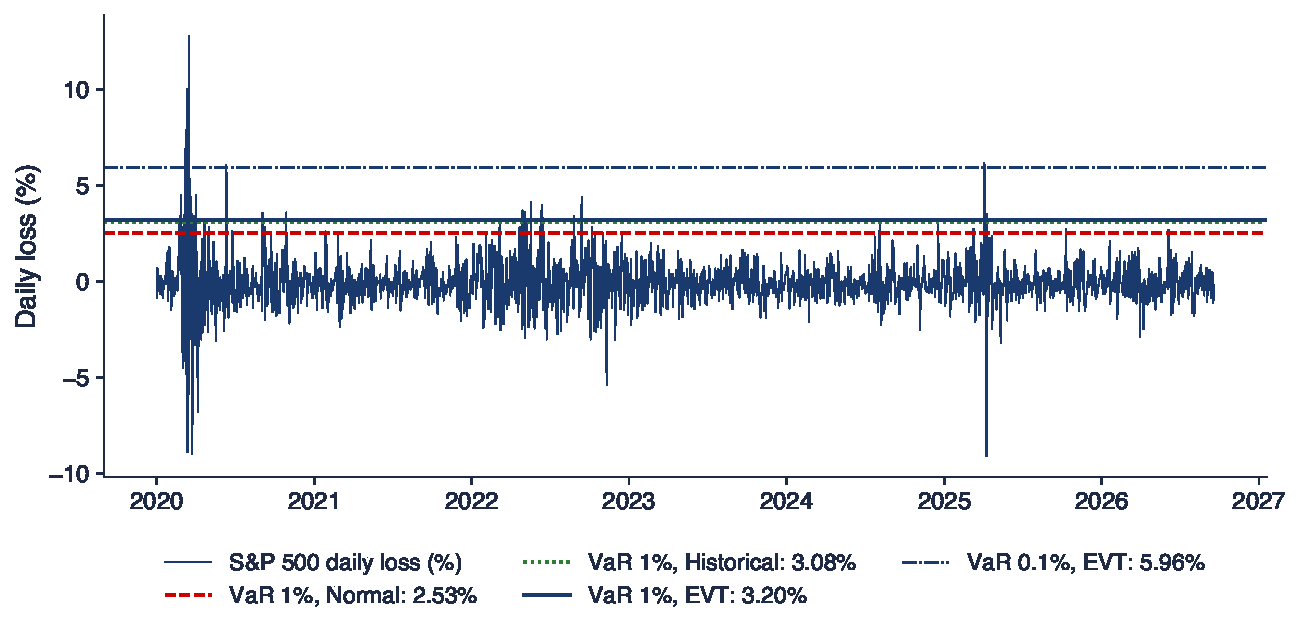
\includegraphics[width=0.97\textwidth,height=0.58\textheight,keepaspectratio]{sfm_ch5_oos.pdf}
\end{center}
\vspace{-0.25cm}
\begin{itemize}
    \item S\&P 500 daily losses after 2019 with the VaR 1\% of the three methods, all estimated on 1990--2019
    \item A good VaR 1\% is exceeded on about 1\% of the test days, here $16.9$ days
\end{itemize}
\quantlet{SFM\_ch5\_evt\_var}{\qlurl{SFM_ch5_evt_var}}
\end{frame}

\begin{frame}{Counting the Exceedances}
\itemsize{\footnotesize}
\begin{center}
\scriptsize
\begin{tabular}{lr|rrrr|rrrr}
\toprule
& & \multicolumn{4}{c|}{VaR 1\%} & \multicolumn{4}{c}{VaR 0.1\%} \\ & test days & expected & EVT & hist. & Normal & expected & EVT & hist. & Normal \\
\midrule
S\&P 500 & 1\,687 & $16.9$ & 25 & 26 & 44 & $1.7$ & 5 & 3 & 23 \\
DAX & 1\,710 & $17.1$ & 15 & 12 & 31 & $1.7$ & 2 & 2 & 8 \\
BET & 1\,674 & $16.7$ & 4 & 5 & 13 & $1.7$ & 0 & 1 & 4 \\
Bitcoin & 2\,453 & $24.5$ & 8 & 10 & 23 & $2.5$ & 1 & 1 & 8 \\
\bottomrule
\end{tabular}
\end{center}
\begin{itemize}
    \item The Normal VaR is exceeded far too often, especially at 0.1\%: 23 days instead of $1.7$ for the S\&P 500
    \item EVT and historical VaR are close to each other; S\&P 500 above the target (the 2020 cluster), BET below it (calm years)
    \item A VaR estimated once ignores the changing volatility: conditional EVT (GARCH + POT) \refMF, Chapters 9 and 10
\end{itemize}\quantlet{SFM\_ch5\_evt\_var}{\qlurl{SFM_ch5_evt_var}}
\end{frame}

\begin{frame}{What EVT Can and Cannot Do}
\itemsize{\small}
\begin{itemize}
    \item \textbf{Can}: give a principled model of the tail and extrapolate beyond the largest observed loss
    \begin{itemize}
        \item stable VaR and ES at 0.1\% where historical simulation has only a handful of points
    \end{itemize}
    \item \textbf{Cannot}: remove the uncertainty of the far tail
    \begin{itemize}
        \item $\hat\xi$ has a standard error of $0.04$--$0.06$ here; return levels beyond the sample have wide intervals
    \end{itemize}
    \item \textbf{Assumes}: i.i.d.\ losses, or at least a stable tail over time
    \begin{itemize}
        \item apply EVT to returns divided by a GARCH volatility (Chapter 9) for daily risk; see also entropy-based ES \refPeleA
    \end{itemize}
    \item Surveys of EVT in finance: \refRocco; \refQRM, Ch.~5
\end{itemize}
\end{frame}

\begin{frame}{Recap: VaR and ES by EVT}
\itemsize{\small}
\begin{itemize}
    \item $\mathrm{VaR}_p = u + \frac{\beta}{\xi}[(np/N_u)^{-\xi} - 1]$; $\mathrm{ES}_p = (\mathrm{VaR}_p + \beta - \xi u)/(1 - \xi)$
    \item VaR 1\% and ES 2.5\%: EVT $\approx$ historical, Normal too low
    \item VaR 0.1\%: EVT about twice the Normal value; historical simulation rests on a few days
    \item Out of sample: the Normal VaR fails; unconditional EVT ignores volatility regimes
\end{itemize}
\end{frame}


%=============================================================================
\section{AI for Scientific Discovery}
%=============================================================================

\begin{frame}{An Open Question}
\itemsize{\small}
\begin{itemize}
    \item \textbf{Has the tail of BET losses changed as the Bucharest market grew?}
    \begin{itemize}
        \item Hill index, $k = 2.5\%$ of $n$: 1997--2009: $\hat\alpha = 2.90$ (block SE $0.33$); 2010--2026: $\hat\alpha = 2.16$ ($0.27$)
        \item $z = -1.73$: a heavier tail after 2010, but not significant at 5\%
    \end{itemize}
    \item Why it is open: the threshold fell from $3.95\%$ to $2.01\%$ with the volatility; is the change in the tail or in the volatility?
    \item AI tools can speed up such a study; they do not replace checking it \refWang
\end{itemize}\quantlet{SFM\_ch5\_hill}{\qlurl{SFM_ch5_hill}}
\end{frame}

\begin{frame}{How AI Could Help}
\itemsize{\small}
\begin{itemize}
    \item \textbf{Literature}: list studies of tail indices in emerging markets and summarise their methods
    \item \textbf{Code}: a first draft of a Hill and POT analysis on rolling windows, with block-bootstrap intervals
    \item \textbf{Robustness}: other thresholds, GARCH-standardised returns, other BVB indices
    \item Example prompt
    \begin{itemize}
        \item \aiprompt{Write a Python function that computes the Hill tail index of daily BET losses with k = 2.5\% of n on rolling 5-year windows, with moving-block bootstrap standard errors (blocks of 20 days).}
    \end{itemize}
\end{itemize}
\end{frame}

\begin{frame}{What to Check}
\itemsize{\small}
\begin{itemize}
    \item Sign: losses are $-r$; a Hill estimate on returns instead of losses measures the gains
    \item Parameterisation: scipy's \texttt{genextreme} uses $c = -\xi$; \texttt{genpareto} uses $c = \xi$
    \item The rule for $k$ or $u$ is fixed before seeing the result, not tuned to get a significant change
    \item Rolling windows overlap: their estimates are not independent tests
    \item References: every cited paper must exist; check the DOI
\end{itemize}
\end{frame}

\begin{frame}{Project Seed}
\itemsize{\small}
\begin{itemize}
    \item \textbf{Question}: is the tail of BET losses lighter or heavier today than before 2010, once volatility is removed?
    \begin{itemize}
        \item data: BET daily closes since 1997 (EODHD); optionally BET-TR since 2014
    \end{itemize}
    \item Steps
    \begin{itemize}
        \item Hill and POT ($u$ at the 90\% quantile) for the two periods, with block-bootstrap intervals
        \item repeat on returns divided by a rolling 60-day volatility: does the difference survive?
        \item compare with the S\&P 500 over the same periods
    \end{itemize}
    \item Deliverable: one table, one chart, and a paragraph on what the data can and cannot show
    \item Declare any AI use, and list the errors of the AI that you corrected
\end{itemize}
\end{frame}


%=============================================================================
\section{Summary}
%=============================================================================

\begin{frame}{Key Takeaways}
\itemsize{\small}
\begin{itemize}
    \item Daily losses have power-law tails with index $\alpha \approx 3$: finite variance, infinite kurtosis
    \item Hill: the tail index from the $k$ largest losses; choose $k$ on the Hill plot; block-bootstrap SE
    \item Block maxima $\to$ GEV; excesses over a threshold $\to$ GPD; the same shape $\xi = 1/\alpha$
    \item Check every fit with mean excess, parameter stability, PP and QQ plots
    \item EVT VaR and ES: close to historical at 1\% and 2.5\%, far above the Normal values at 0.1\%
    \item Extrapolation far beyond the data remains uncertain: report intervals
\end{itemize}
\end{frame}

\begin{frame}{Key Formulas}
\itemsize{\small}
{\renewcommand{\arraystretch}{1.45}\begin{center}
\scriptsize
\begin{tabular}{ll}
\toprule
\textbf{Quantity} & \textbf{Formula} \\
\midrule
Regular variation & $P(L > x) = x^{-\alpha}\ell(x)$, \quad $P(L > tx)/P(L > x) \to t^{-\alpha}$ \\
Hill & $\hat\alpha_k = [\frac1k\sum_{i=1}^k \ln(L_{(i)}/L_{(k+1)})]^{-1}$, \quad $\mathrm{SE} \approx \hat\alpha/\sqrt{k}$ \\
Hill quantile & $\hat x_p = L_{(k+1)}(k/(np))^{1/\hat\alpha}$ \\
Mean excess & $e(u) = E[L - u \mid L > u]$; \quad GPD: $(\beta + \xi(v - u))/(1 - \xi)$ \\
GEV & $H(x) = \exp\{-[1 + \xi(x - \mu)/\sigma]^{-1/\xi}\}$ \\
Return level & $z_T = \mu + \frac{\sigma}{\xi}[(-\ln(1 - \frac{1}{12T}))^{-\xi} - 1]$ \\
GPD & $G(y) = 1 - (1 + \xi y/\beta)^{-1/\xi}$ \\
VaR (POT) & $u + \frac{\beta}{\xi}[(np/N_u)^{-\xi} - 1]$ \\
ES (POT) & $(\mathrm{VaR}_p + \beta - \xi u)/(1 - \xi)$ \\
\bottomrule
\end{tabular}
\end{center}
}
\end{frame}

\begin{frame}{Check Yourself}
\itemsize{\small}
\begin{itemize}
    \item \textbf{Question}: a GPD fit gives $\hat\xi = 0.25$; which moments of the losses exist?
    \begin{itemize}
        \item \textbf{Answer}: $\alpha = 1/\xi = 4$: mean, variance and skewness exist; the kurtosis does not ($m < 4$ only)
    \end{itemize}
    \item \textbf{Question}: why use the 2.5\% largest losses and not all losses for the Hill estimator?
    \begin{itemize}
        \item \textbf{Answer}: the power law holds only in the tail; with the body included $\hat\alpha$ is biased
    \end{itemize}
    \item \textbf{Question}: is VaR 0.1\% by historical simulation reliable with 10 years of data?
    \begin{itemize}
        \item \textbf{Answer}: no: about 2\,500 days leave only 2--3 losses beyond it; EVT uses the whole tail
    \end{itemize}
    \item Next: \sfmchlink{https://danpele.github.io/SFM/EN/Courses/chapter6_model_selection_risk_management.pdf}{Chapter 6}, model selection and risk management
\end{itemize}
\end{frame}


%=============================================================================
\section{References}
%=============================================================================

\begin{frame}{References (1/2)}
\itemsize{\tiny}
\begin{itemize}
    \item Acerbi, C., Tasche, D. (2002). \href{https://doi.org/10.1016/S0378-4266(02)00283-2}{On the coherence of expected shortfall}. \textit{Journal of Banking \& Finance}, 26(7), 1487--1503.
    \item Balkema, A.A., de Haan, L. (1974). \href{https://doi.org/10.1214/aop/1176996548}{Residual life time at great age}. \textit{Annals of Probability}, 2(5), 792--804.
    \item Basel Committee on Banking Supervision. \href{https://www.bis.org/basel_framework/chapter/MAR/33.htm}{MAR33: Internal models approach -- capital requirements calculation}. \textit{The Basel Framework}. Bank for International Settlements.
    \item Borak, S., Härdle, W.K., López-Cabrera, B. (2013). \href{https://doi.org/10.1007/978-3-642-33929-5}{\textit{Statistics of Financial Markets: Exercises and Solutions}}, 2nd ed. Springer.
    \item Carlson, M. (2007). \href{https://www.federalreserve.gov/pubs/feds/2007/200713/200713pap.pdf}{A brief history of the 1987 stock market crash with a discussion of the Federal Reserve response}. \textit{Finance and Economics Discussion Series} 2007-13, Board of Governors of the Federal Reserve System.
    \item Coles, S. (2001). \href{https://doi.org/10.1007/978-1-4471-3675-0}{\textit{An Introduction to Statistical Modeling of Extreme Values}}. Springer.
    \item Cont, R. (2001). \href{https://doi.org/10.1080/713665670}{Empirical properties of asset returns: stylized facts and statistical issues}. \textit{Quantitative Finance}, 1(2), 223--236.
    \item Daníelsson, J., de Vries, C.G. (1997). \href{https://doi.org/10.1016/S0927-5398(97)00008-X}{Tail index and quantile estimation with very high frequency data}. \textit{Journal of Empirical Finance}, 4(2--3), 241--257.
    \item Davison, A.C., Smith, R.L. (1990). \href{https://doi.org/10.1111/j.2517-6161.1990.tb01796.x}{Models for exceedances over high thresholds}. \textit{Journal of the Royal Statistical Society, Series B}, 52(3), 393--425.
    \item Drees, H., Resnick, S., de Haan, L. (2000). \href{https://doi.org/10.1214/aos/1016120372}{How to make a Hill plot}. \textit{Annals of Statistics}, 28(1), 254--274.
    \item Embrechts, P., Klüppelberg, C., Mikosch, T. (1997). \href{https://doi.org/10.1007/978-3-642-33483-2}{\textit{Modelling Extremal Events for Insurance and Finance}}. Springer.
    \item Fisher, R.A., Tippett, L.H.C. (1928). \href{https://doi.org/10.1017/S0305004100015681}{Limiting forms of the frequency distribution of the largest or smallest member of a sample}. \textit{Mathematical Proceedings of the Cambridge Philosophical Society}, 24(2), 180--190.
    \item Franke, J., Härdle, W.K., Hafner, C.M. (2019). \href{https://doi.org/10.1007/978-3-030-13751-9}{\textit{Statistics of Financial Markets: An Introduction}}, 5th ed. Springer.
    \item Gnedenko, B. (1943). \href{https://doi.org/10.2307/1968974}{Sur la distribution limite du terme maximum d'une série aléatoire}. \textit{Annals of Mathematics}, 44(3), 423--453.
    \item Gopikrishnan, P., Plerou, V., Amaral, L.A.N., Meyer, M., Stanley, H.E. (1999). \href{https://doi.org/10.1103/PhysRevE.60.5305}{Scaling of the distribution of fluctuations of financial market indices}. \textit{Physical Review E}, 60(5), 5305--5316.
    \item Gumbel, E.J. (1958). \href{https://doi.org/10.7312/gumb92958}{\textit{Statistics of Extremes}}. Columbia University Press.
\end{itemize}
\end{frame}

\begin{frame}{References (2/2)}
\itemsize{\tiny}
\begin{itemize}
    \item Hill, B.M. (1975). \href{https://doi.org/10.1214/aos/1176343247}{A simple general approach to inference about the tail of a distribution}. \textit{Annals of Statistics}, 3(5), 1163--1174.
    \item Jansen, D.W., de Vries, C.G. (1991). \href{https://doi.org/10.2307/2109682}{On the frequency of large stock returns: putting booms and busts into perspective}. \textit{Review of Economics and Statistics}, 73(1), 18--24.
    \item Jenkinson, A.F. (1955). \href{https://doi.org/10.1002/qj.49708134804}{The frequency distribution of the annual maximum (or minimum) values of meteorological elements}. \textit{Quarterly Journal of the Royal Meteorological Society}, 81(348), 158--171.
    \item Longin, F.M. (1996). \href{https://doi.org/10.1086/209695}{The asymptotic distribution of extreme stock market returns}. \textit{Journal of Business}, 69(3), 383--408.
    \item Mandelbrot, B. (1963). \href{https://doi.org/10.1086/294632}{The variation of certain speculative prices}. \textit{Journal of Business}, 36(4), 394--419.
    \item McNeil, A.J., Frey, R. (2000). \href{https://doi.org/10.1016/S0927-5398(00)00012-8}{Estimation of tail-related risk measures for heteroscedastic financial time series: an extreme value approach}. \textit{Journal of Empirical Finance}, 7(3--4), 271--300.
    \item McNeil, A.J., Frey, R., Embrechts, P. (2015). \href{https://press.princeton.edu/books/hardcover/9780691166278/quantitative-risk-management}{\textit{Quantitative Risk Management: Concepts, Techniques and Tools}}, revised ed. Princeton University Press.
    \item Pele, D.T., Lazar, E., Dufour, A. (2017). \href{https://doi.org/10.3390/e19050226}{Information entropy and measures of market risk}. \textit{Entropy}, 19(5), 226.
    \item Pele, D.T., Lazar, E., Mazurencu-Marinescu-Pele, M. (2019). \href{https://doi.org/10.3390/e21121204}{Modeling expected shortfall using tail entropy}. \textit{Entropy}, 21(12), 1204.
    \item Pickands, J. (1975). \href{https://doi.org/10.1214/aos/1176343003}{Statistical inference using extreme order statistics}. \textit{Annals of Statistics}, 3(1), 119--131.
    \item Resnick, S.I. (2007). \href{https://doi.org/10.1007/978-0-387-45024-7}{\textit{Heavy-Tail Phenomena: Probabilistic and Statistical Modeling}}. Springer.
    \item Rocco, M. (2014). \href{https://doi.org/10.1111/j.1467-6419.2012.00744.x}{Extreme value theory in finance: a survey}. \textit{Journal of Economic Surveys}, 28(1), 82--108.
    \item Wang, H., Fu, T., Du, Y., Gao, W., et al. (2023). \href{https://doi.org/10.1038/s41586-023-06221-2}{Scientific discovery in the age of artificial intelligence}. \textit{Nature}, 620, 47--60.
    \item Weissman, I. (1978). \href{https://doi.org/10.1080/01621459.1978.10480104}{Estimation of parameters and large quantiles based on the $k$ largest observations}. \textit{Journal of the American Statistical Association}, 73(364), 812--815.
\end{itemize}
\end{frame}

\end{document}
